\chapter{同伦类型论 (Homotopy Type Theory)}
\label{cha:basics}

同伦类型论中的一个核心新观点是,可以将类型视为同伦理论中的空间或范畴论中的高维群胚(higher-dimensional groupoids)。

\index{classical!homotopy theory|(}
\index{higher category theory|(}
我们首先简要介绍同伦理论与高维范畴论之间的联系。
在经典同伦理论中,空间 $X$ 是一组带有拓扑结构的点集合,
\indexsee{space!topological}{topological space}
\index{topological!space}
而点 $x$ 和 $y$ 之间的路径通过一个连续映射 $p : [0,1] \to X$ 来表示,其中 $p(0) = x$ 和 $p(1) = y$。
\index{path!topological}
\index{topological!path}
这个函数可以被视为在每一个“时间点”提供 $X$ 中的一个点。对于许多目的而言,路径的严格相等(即逐点相等的函数)是一个过于精细的概念。例如,可以定义路径拼接操作(如果 $p$ 是从 $x$ 到 $y$ 的路径,$q$ 是从 $y$ 到 $z$ 的路径,那么拼接 $p \ct q$ 是从 $x$ 到 $z$ 的路径)和逆操作($\opp p$ 是从 $y$ 到 $x$ 的路径)。然而,这些操作之间存在自然的等式,但对于严格相等来说并不成立:例如,路径 $p \ct \opp p$(从 $x$ 走到 $y$,然后沿同一路径返回,时间从 $0$ 走到 $1$)并不严格等于恒等路径(在所有时间点都停留在 $x$ 处)。

解决方法是考虑一种称为\emph{同伦 (homotopy)}的路径相等的更粗略概念。
\index{homotopy!topological}
两个连续映射 $f : X_1 \to X_2$ 和 $g : X_1 \to X_2$ 之间的同伦是一个连续映射 $H : X_1 \times [0, 1] \to X_2$,满足 $H(x, 0) = f(x)$ 和 $H(x, 1) = g(x)$。在从 $x$ 到 $y$ 的路径 $p$ 和 $q$ 的特定情况下,同伦是一个连续映射 $H : [0,1] \times [0,1] \rightarrow X$,使得对所有 $s\in [0,1]$,$H(s,0) = p(s)$ 和 $H(s,1) = q(s)$。
在这种情况下,我们还要求对所有 $t\in [0,1]$,$H(0,t) = x$ 和 $H(1,t)=y$,以使得对每个 $t$,函数 $H(\blank,t)$ 再次是从 $x$ 到 $y$ 的路径;这种类型的同伦被称为\emph{端点保持 (endpoint-preserving)}或\emph{相对端点 (rel endpoints)}。
在简单的情况下,我们可以将 $H$ 的方形 $[0,1]\times [0,1]$ 的映像视为“填充”在 $p$ 和 $q$ 之间的空间,尽管对于一般的 $X$ 来说,这并不实际;更好的是将 $H$ 视为将 $p$ 连续变形为 $q$ 的过程,且不移动端点。
由于 $[0,1]\times [0,1]$ 是二维的,我们也可以称 $H$ 为路径之间的二维\emph{路径 (2-dimensional path)}。\index{path!2-}

例如,由于 $p \ct \opp p$ 沿同一路径来回走,你知道你可以将 $p \ct \opp p$ 连续缩小到恒等路径——例如,它不会被空间中的一个洞卡住。
同伦是一个等价关系,并且诸如拼接、逆操作等操作都尊重同伦。此外,在某个点 $x_0$ 处的闭环的同伦等价类(其中两个闭环 $p$ 和 $q$ 在它们之间存在\emph{基点保持 (based)}同伦时被等同,这是一种满足 $H(0,t) = H(1,t) = x_0$ 的同伦)形成一个称为\emph{基本群 (fundamental group)}的群。\index{fundamental!group}这个群是空间的一个\emph{代数不变量 (algebraic invariant)},可以用来调查两个空间是否\emph{同伦等价 (homotopy equivalent)}(存在来回连续映射且它们的复合是同伦于恒等映射的),因为等价空间具有同构的基本群。

由于同伦本身是一种二维路径,因此自然存在三维\emph{同伦之间的同伦 (homotopy between homotopies)}\index{path!3-},然后是\emph{同伦之间的同伦之间的同伦},依此类推。
这个由点、路径、同伦、同伦之间的同伦……所组成的无限塔,带有诸如基本群的代数操作,是一种称为\emph{(弱)$\infty$-群胚 (weak $\infty$-groupoid)}的代数结构。\index{.infinity-groupoid@$\infty$-groupoid} $\infty$-群胚\index{.infinity-groupoid@$\infty$-groupoid}包含一组对象,然后是对象之间的\emph{态射 (morphisms)}\indexdef{morphism!in an .infinity-groupoid@in an $\infty$-groupoid},然后是态射之间的\emph{态射},依此类推,并带有一些复杂的代数结构;在每一层级上的态射称为\define{$k$-态射 ($k$-morphism)}。\indexdef{k-morphism@$k$-morphism}每一层级的态射具有恒等、组合和逆操作,这些操作在某种意义上是弱的,即它们仅满足到下一层级的态射的群胚定律(组合的结合律、恒等是组合的单位元、逆元素消除),而这种弱性导致了进一步的结构。例如,由于组合的结合律 $p \ct (q \ct r) = (p \ct q) \ct r$ 本身是一种高维态射,因此需要额外的操作来关联各种结合律的证明:将 $p \ct (q \ct (r \ct s))$ 重新组合成 $((p \ct q) \ct r) \ct s$ 的各种方式产生了 Mac Lane 的五边形。\index{pentagon, Mac Lane}这种弱性还在各个层级之间产生了非平凡的相互作用。

每一个拓扑空间 $X$ 都具有一个\emph{基本$\infty$-群胚 (fundamental $\infty$-groupoid)},\index{.infinity-groupoid@$\infty$-groupoid!fundamental}\index{fundamental!.infinity-groupoid@$\infty$-groupoid}其 $k$-态射是 $X$ 中的 $k$维路径。$\infty$-群胚的弱性直接对应于路径仅同伦的事实,$(k+1)$-路径充当 $k$-路径之间的同伦。此外,将空间视为 $\infty$-群胚保持了足够的空间方面的特征以进行同伦理论:基本 $\infty$-群胚构造与 $\infty$-群胚作为空间的几何实现是伴随的,并且这种伴随保持了同伦理论(这被称为\emph{同伦假设/定理 (homotopy hypothesis/theorem)},\index{hypothesis!homotopy}\index{homotopy!hypothesis}因为它是一个假设还是定理取决于你如何定义 $\infty$-群胚)。例如,你可以很容易地定义一个 $\infty$-群胚的基本群,如果你计算一个空间的基本 $\infty$-群胚的基本群,它将与该空间的经典基本群的定义一致。由于这种对应关系,同伦理论与高维范畴论紧密相关。

\index{classical!homotopy theory|)}%
\index{higher category theory|)}%

\mentalpause

现在,在同伦类型论中,每一个类型都可以被视为具有 $\infty$-群胚的结构。回想一下,对于任何类型 $A$,以及任何 $x,y:A$,我们有一个等同性类型 $\id[A]{x}{y}$,也可以写作 $\idtype[A]{x}{y}$ 或简单地写作 $x=y$。从逻辑上讲,我们可以将 $\id[A]{x}{y}$ 的元素视为 $x$ 和 $y$ 相等的证据,或者是 $x$ 与 $y$ 的同一化(identification)。此外,类型论(不同于一阶逻辑)允许我们将 $\id[A]{x}{y}$ 的元素也视为可以成为进一步命题的对象的个体。因此,我们可以\emph{迭代}等同性类型:我们可以形成同一化 $p,q$ 之间的 $\id[{(\id[A]{x}{y})}]{p}{q}$ 类型,以及同一化 $r,s$ 之间的 $\id[{(\id[{(\id[A]{x}{y})}]{p}{q})}]{r}{s}$ 类型,依此类推。这种等同性类型的层级结构与空间中的连续路径及其之间的(更高阶)同伦,或一个 $\infty$-群胚的结构完全对应。\index{.infinity-groupoid@$\infty$-groupoid}

因此,我们经常将一个元素 $p : \id[A]{x}{y}$ 称为从 $x$ 到 $y$ 的\define{路径 (path)},\index{path}称 $x$ 为其\define{起点 (start point)},\indexdef{start point of a path}\indexdef{path!start point of}称 $y$ 为其\define{终点 (end point)}。\indexdef{end point of a path}\indexdef{path!end point of} 具有相同起点和终点的两条路径 $p,q : \id[A]{x}{y}$ 称为\define{平行 (parallel)},\indexdef{parallel paths}\indexdef{path!parallel}在这种情况下,元素 $r : \id[{(\id[A]{x}{y})}]{p}{q}$ 可以被视为同伦,或者是态射之间的态射;我们通常称它为\define{二维路径 (2-path)}\indexdef{path!2-}\indexsee{2-path}{path, 2-}或\define{二维路径 (2-dimensional path)}。\index{dimension!of paths}\indexsee{2-dimensional path}{path, 2-}\indexsee{path!2-dimensional}{path, 2-}类似地,$\id[{(\id[{(\id[A]{x}{y})}]{p}{q})}]{r}{s}$ 是\define{三维路径 (3-dimensional paths)}\indexdef{path!3-}\indexsee{3-path}{path, 3-}\indexsee{3-dimensional path}{path, 3-}\indexsee{path!3-dimensional}{path, 3-}的类型,用于两个平行二维路径之间的同一化。 如果类型 $A$ 是“类集(set-like)”的,如 \nat,这些迭代的等同性类型将变得无趣(参见 \cref{sec:basics-sets}),但在一般情况下,它们可以建模非平凡的同伦类型。

%% (显然,“$\id[A]{x}{y}$” 的符号在这里有其局限性。样式 $\idtype[A]{x}{y}$ 在迭代中只稍微好一些:$\idtype[{\idtype[{\idtype[A]{x}{y}}]{p}{q}}]{r}{s}$。)

同伦类型论与经典同伦理论之间的一个重要区别在于,同伦类型论提供了一种\emph{综合的 (synthetic)}描述空间的方式,\index{synthetic mathematics}\index{geometry, synthetic}\index{Euclid of Alexandria}如下所示。综合几何是欧几里得(Euclid)风格的几何学~\cite{Euclid}:从一些基本概念(点和线)、构造(连接任何两点的线)和公理(所有直角都相等)开始,逻辑地推导出结论。这与解析几何形成对比,\index{analytic mathematics}其中点和线等概念用 $\R^n$ 中的笛卡尔坐标具体表示——线是点集——并且基本的构造和公理源自这种表示。虽然经典同伦理论是解析性的(空间和路径是由点构成的),同伦类型论是综合性的:点、路径及路径之间的路径是基本的、不可分割的、原始的概念。

此外,同伦类型论的一个令人惊叹之处在于,所有基本的构造和公理——所有更高维的群胚结构——都自动从等同性类型的归纳原理中产生。
回想 \cref{sec:identity-types} 中的内容,该内容表明如果
\begin{itemize}
  \item 对于每个 $x,y:A$ 以及每个 $p:\id[A]xy$,我们有一个类型 $D(x,y,p)$,并且
  \item 对于每个 $a:A$,我们有一个元素 $d(a):D(a,a,\refl a)$,
\end{itemize}
那么
\begin{itemize}
  \item 对于\emph{每}个元素 $x,y:A$ 及 $p:\id[A]xy$,存在一个元素 $\indid{A}(D,d,x,y,p):D(x,y,p)$,使得 $\indid{A}(D,d,a,a,\refl a) \jdeq d(a)$。
\end{itemize}
换句话说,给定依赖函数
\begin{align*}
  D & :\prd{x,y:A} (\id{x}{y}) \to \type\\
  d & :\prd{a:A} D(a,a,\refl{a})
\end{align*}
存在一个依赖函数
\[\indid{A}(D,d):\prd{x,y:A}{p:\id{x}{y}} D(x,y,p)\]
使得
\begin{equation}\label{eq:Jconv}
\indid{A}(D,d,a,a,\refl{a})\jdeq d(a)
\end{equation}
对于每个 $a:A$。
通常,每当我们应用这个归纳规则时,我们要么不关心正在定义的特定函数,要么会立即给它一个不同的名称。

非正式地说,等同性类型的归纳原理表明,如果我们想要构造一个依赖于等同性类型的居住者 $p:\id[A]xy$ 的对象(或证明一个命题),那么仅在 $x$ 和 $y$ 是相同的(判断上的)且 $p$ 是反身元素 $\refl{x}:x=x$(判断上的)时进行构造(或证明)就足够了。
在非正式书写时,我们可能会用类似“通过归纳,可以假设……”的短语来表达这一点。
这种对“反身情况”的简化类似于在自然数上的归纳证明中的“基例”和“归纳步骤”的简化,也类似于在不交并或析取上的例证证明中的“左例证”和“右例证”的简化。\index{induction principle!for identity type}%

在自然数上的归纳证明的背景下,“转换规则”~\eqref{eq:Jconv} 并不常见,但在递归定义的相关概念中存在类似的概念。
如果一个序列 $(a_n)_{n\in \mathbb{N}}$ 是通过给定 $a_0$ 并根据 $a_n$ 指定 $a_{n+1}$ 来定义的,那么实际上生成序列的 $0^{\mathrm{th}}$ 项\emph{就是}给定的,并且给定的递推关系在生成的序列上成立。
(这似乎显而易见,不值得一提,但如果我们将递归定义视为计算序列值的算法\index{algorithm},那么这正是执行该算法的过程。)
规则~\eqref{eq:Jconv} 是类比的:它表明,如果我们通过指定当 $p$ 是 $\refl{x}:x=x$ 时的值来为所有 $p:x=y$ 定义一个对象 $f(p)$,那么我们指定的值实际上就是 $f(\refl{x})$ 的值。

这个归纳原理赋予每个类型 $\infty$-群胚\index{.infinity-groupoid@$\infty$-groupoid}的结构,并且每个类型之间的函数都具有 $\infty$-函子\index{.infinity-functor@$\infty$-functor}之间的函子的结构。这从数学的角度来看很有趣,因为它提供了一种处理 $\infty$-群胚的新方式。这从类型理论的角度来看也很有趣,因为它揭示了与每个类型和函数相关的新操作。在本章的其余部分,我们将开始探索这个结构。

\section{类型是高阶群体 (Types are higher groupoids)}
\label{sec:equality}

\index{类型!等同|(type!identity|(}%
\index{路径|(path|(}%
\index{.无穷群体@$\infty$-群体!类型的结构|(structure of a type|(}%
我们现在从归纳原理推导出高阶群体结构的开端。我们从等同的对称性开始,在拓扑语言中,这意味着“路径可以反向”。

\begin{lem}\label{lem:opp}
对于每一个类型 $A$ 和每一个 $x,y:A$,存在一个函数
\begin{equation*}
(x= y)\to(y= x)
\end{equation*}
记作 $p\mapsto \opp{p}$,使得对每一个 $x:A$,有 $\opp{\refl{x}}\jdeq\refl{x}$。我们称 $\opp{p}$ 为 $p$ 的 \define{逆元 (inverse)}。
\indexdef{路径!逆元 (path!inverse)}%
\indexdef{逆元!路径的 (inverse!of path)}%
\index{等同性!对称性 (equality!symmetry of)}%a
\index{对称性!等同性的 (symmetry!of equality)}%
\end{lem}

因为这是我们第一次声明某个东西为“引理”或“定理”,让我们停下来考虑一下这意味着什么。回想一下,命题(可以被证明的陈述)与类型等同,而引理和定理(已经被证明的陈述)与 \emph{居住的 (inhabited)} 类型等同。因此,引理或定理的陈述应被翻译成一个类型,如 \cref{sec:pat} 中那样,其证明被翻译成该类型的一个居住者。根据全称量词“对于每一个”的解释,\cref{lem:opp} 对应的类型是
\[ \prd{A:\UU}{x,y:A} (x= y)\to(y= x). \]
\cref{lem:opp} 的证明将包含构建该类型的一个元素,即推导出某个 $f:\prd{A:\UU}{x,y:A} (x= y)\to(y= x)$ 的判断。然后我们为这个元素 $f$ 引入符号 $\opp{(\blank)}$,其中 $A$、$x$ 和 $y$ 的参数被省略并从上下文推断。(如在 \cref{sec:types-vs-sets} 中所述,次要陈述“对于每一个 $x:A$,有 $\opp{\refl{x}}\jdeq\refl{x}$”应该被视为一个单独的判断。)

\begin{proof}[第一个证明 (First proof)]
  假设给定 $A:\UU$,
  令 $D:\prd{x,y:A}(x= y) \to \type$ 为由 $D(x,y,p)\defeq (y= x)$ 定义的类型族。换句话说,$D$ 是一个函数,将任意 $x,y:A$ 和 $p:x=y$ 分配给一个类型,即类型 $y=x$。然后我们有一个元素
  \begin{equation*}
    d\defeq \lam{x} \refl{x}:\prd{x:A} D(x,x,\refl{x}).
  \end{equation*}
  因此,身份类型的归纳原理给我们提供了一个元素
  \narrowequation{ \indid{A}(D,d,x,y,p): (y= x)}
  对于每个 $p:(x= y)$。我们现在可以定义所需的函数 $\opp{(\blank)}$ 为 $\lam{p} \indid{A}(D,d,x,y,p)$,即我们设 $\opp{p} \defeq \indid{A}(D,d,x,y,p)$。
  转换规则~\eqref{eq:Jconv} 给出 $\opp{\refl{x}}\jdeq \refl{x}$,如所需。
\end{proof}

我们以非常形式化的风格写出了这个证明,这在身份类型的归纳规则不熟悉时可能会有所帮助。为了更正式,我们可以说 \cref{lem:opp} 及其证明共同构成了以下判断
\begin{narrowmultline*}
  \lam{A}{x}{y}{p} \indid{A}((\lam{x}{y}{p} (y=x)), (\lam{x} \refl{x}), x, y, p)
  \narrowbreak : \prd{A:\UU}{x,y:A} (x= y)\to(y= x)
\end{narrowmultline*}
(以及额外的等同性判断)。然而,最终我们更喜欢使用更自然的语言,如以下等效的证明中那样。

\begin{proof}[第二个证明 (Second proof)]
  我们希望为每个 $x,y:A$ 和 $p:x=y$ 构造一个元素 $\opp{p}:y=x$。通过归纳,我们只需在 $y$ 为 $x$ 并且 $p$ 为 $\refl{x}$ 的情况下完成此操作。但在这种情况下,$p$ 的类型 $x=y$ 和我们试图构造 $\opp{p}$ 的类型 $y=x$ 都只是 $x=x$。因此,在“反射性情况”中,我们可以将 $\opp{\refl{x}}$ 简单地定义为 $\refl{x}$。然后通过归纳原理得出一般情况,并且转换规则 $\opp{\refl{x}}\jdeq\refl{x}$ 正是我们在反射性情况中给出的证明。
\end{proof}

我们将以这两种风格写出接下来的几个证明,以帮助读者熟悉后一种风格。接下来我们证明等同性的传递性,或等价地,我们“连接路径”。

\begin{lem}\label{lem:concat}
对于每一个类型 $A$ 和每一个 $x,y,z:A$,存在一个函数
\begin{equation*}
(x= y) \to   (y= z)\to (x=  z),
\end{equation*}
写作 $p \mapsto q \mapsto p\ct q$,使得对于任意 $x:A$,$\refl{x}\ct \refl{x}\jdeq \refl{x}$。
我们称 $p\ct q$ 为 $p$ 和 $q$ 的 \define{连接 (concatenation)} 或 \define{复合 (composite)}。
\indexdef{路径!连接 (path!concatenation)}%
\indexdef{路径!复合 (path!composite)}%
\indexdef{路径连接 (concatenation of paths)}%
\indexdef{路径的复合 (composition!of paths)}%
\index{等同性!传递性 (equality!transitivity of)}%
\index{传递性!等同性的 (transitivity!of equality)}%
\end{lem}

注意,我们选择以与函数复合相反的顺序来表示路径连接:从 $p:x=y$ 和 $q:y=z$ 我们得到 $p\ct q : x=z$,而从 $f:A\to B$ 和 $g:B\to C$ 我们得到 $g\circ f : A\to C$(见 \cref{ex:composition})。

\begin{proof}[第一个证明 (First proof)]
  所需的函数类型为 $\prd{x,y,z:A} (x= y) \to   (y= z)\to (x=  z)$。
  我们将定义一个具有等效类型的函数 $\prd{x,y:A} (x= y) \to \prd{z:A} (y= z)\to (x=  z)$,这允许我们进行两次路径归纳。令 $D:\prd{x,y:A} (x=y) \to \type$ 为类型族
  \begin{equation*}
    D(x,y,p)\defeq \prd{z:A}{q:y=z} (x=z)。
  \end{equation*}
  注意 $D(x,x,\refl x) \jdeq \prd{z:A}{q:x=z} (x=z)$。
  因此,为了将身份类型的归纳原理应用于此 $D$,我们需要一个类型为
  \begin{equation}\label{eq:concatD}
  \prd{x:A} D(x,x,\refl{x})
  \end{equation}
  的函数,即类型为
  \[ \prd{x,z:A}{q:x=z} (x=z)。\]
  现在令 $E:\prd{x,z:A}{q:x=z}\type$ 为类型族 $E(x,z,q)\defeq (x=z)$。
  注意 $E(x,x,\refl x) \jdeq (x=x)$。
  因此,我们有函数
  \begin{equation*}
    e(x) \defeq \refl{x} : E(x,x,\refl{x})。
  \end{equation*}
  通过身份类型的归纳原理应用于 $E$,我们得到一个函数
  \begin{equation*}
    d : \prd{x,z:A}{q:x=z} E(x,z,q)。
  \end{equation*}
  但是 $E(x,z,q)\jdeq (x=z)$,所以 $d$ 的类型是~\eqref{eq:concatD}。
  因此,我们可以使用此函数 $d$ 并将身份类型的归纳原理应用于 $D$,以获得我们所需的函数类型
  \begin{equation*}
    \prd{x,y:A} (x= y) \to \prd{z:A} (y= z)\to (x=  z)
  \end{equation*}
  因此 $\prd{x,y,z:A} (y=z) \to (x=y) \to (x=z)$。
  两个归纳原理的转换规则为任意 $x:A$ 给出了 $\refl{x}\ct \refl{x}\jdeq \refl{x}$。
\end{proof}

\begin{proof}[第二个证明 (Second proof)]
  我们希望为每个 $x,y,z:A$ 和每个 $p:x=y$ 和 $q:y=z$ 构造一个 $x=z$ 的元素。
  通过对 $p$ 进行归纳,我们只需假设 $y$ 是 $x$ 并且 $p$ 是 $\refl{x}$。
  在这种情况下,$q$ 的类型 $y=z$ 是 $x=z$。
  现在通过对 $q$ 进行归纳,我们只需再假设 $z$ 是 $x$ 并且 $q$ 是 $\refl{x}$。
  但在这种情况下,$x=z$ 是 $x=x$,我们有 $\refl{x}:(x=x)$。
\end{proof}

读者可能会觉得我们给出的这个引理证明过于复杂。实际上,我们可以在对 $p$ 进行归纳后停止,因为此时我们要生成的是一个等同 $x=z$,而我们已经有这样的等同,即 $q$。为什么我们还要继续对 $q$ 进行另一个归纳?

答案是,如介绍中所述,我们正在做的是 \emph{证明相关的 (proof-relevant)} 数学。
\index{数学!证明相关 (mathematics!proof-relevant)}%
当我们证明一个引理时,我们是在定义某个类型的一个居住者,并且在证明过程中定义的具体元素可能很重要,而不仅仅是该元素所居住的类型(即引理的 \emph{陈述})。\cref{lem:concat} 有三个显而易见的证明:我们可以对 $p$ 进行归纳,对 $q$ 进行归纳,或对它们进行双重归纳。如果我们用三种不同的方式证明它,我们将有三个相同类型的不同元素。不难证明这三个元素是相等的(见 \cref{ex:basics:concat}),但由于它们并非 \emph{定义上} 相等,因此可能仍有理由偏爱其中之一。

在 \cref{lem:concat} 的情况下,差异取决于计算规则。如果我们使用单一归纳对 $p$ 证明引理,那么我们将得到形式为 $\refl{y} \ct q \jdeq q$ 的计算规则。如果我们使用单一归纳对 $q$ 证明,那么我们将得到 $p\ct\refl{y}\jdeq p$,而我们用双重归纳(如我们所做的)证明则仅得到 $\refl{x}\ct\refl{x} \jdeq \refl{x}$。

\index{数学!形式化 (mathematics!formalized)}%
不对称的计算规则有时在做形式化数学时很方便,因为它们允许计算机自动简化更多内容。然而,在非正式数学中,甚至在形式化情况下,拥有一个表现不对称的连接操作并且必须记住哪个侧面是“特殊”的,可能会让人困惑。对两侧进行对称处理可以使证明更具稳健性;这就是为什么我们给出了我们所做的证明。(然而,这无疑是一个风格上的选择。)

下表总结了我们迄今为止所做的“等同性”、“同伦”和“高阶群体”的观点。
\begin{center}
  \medskip
  \begin{tabular}{ccc}
    \toprule
    等同性 (Equality) & 同伦 (Homotopy) & $\infty$-群体 ($\infty$-Groupoid)\\
    \midrule
    反射性\index{等同性!反射性 (equality!reflexivity of)} & 常量路径 & 恒等态射\\
    对称性\index{等同性!对称性 (equality!symmetry of)} & 路径反转 & 逆态射\\
    传递性\index{等同性!传递性 (equality!transitivity of)} & 路径连接 & 态射复合\\
    \bottomrule
  \end{tabular}
  \medskip
\end{center}

在实践中,传递性通常用于通过一系列中间步骤证明一个等同。我们将使用常见的符号表示,例如 $a=b=c=d$。如果中间表达式较长,或者我们想要指定每个等同的证据,我们可以写
\begin{align*}
  a &= b & \text{(由 $p$)}\\ &= c &\text{(由 $q$)} \\ &= d &\text{(由 $r$)}。
\end{align*}
在任何一种情况下,该符号表示构造元素 $(p\ct q)\ct r: (a=d)$。(为了具体化,我们选择左结合性,尽管考虑到 \cref{thm:omg}\ref{item:omg4},这几乎没有区别。)如果发生 $b$ 和 $c$ 是判断上相等的情况,那么我们可以写
\begin{align*}
  a &= b & \text{(由 $p$)}\\ &\jdeq c \\ &= d &\text{(由 $r$)}
\end{align*}
来表示构造 $p\ct r : (a=d)$。我们还遵循常见的数学实践,不要求该符号中的正当理由(“由 $p$”和“由 $r$”)提供所需的确切证据;相反,我们允许它们简单地提及构造该证据时最重要(或最不明显)的成分。例如,如果“引理 A”声明对于所有 $x$ 和 $y$ 我们有 $f(x)=g(y)$,那么我们可以写“由引理 A”作为步骤 $f(a) = g(b)$ 的正当理由,并相信读者能够推断出我们将引理 A 应用于 $x\defeq a$ 和 $y\defeq b$。如果我们相信读者能够猜出正当理由,我们也可以完全省略一个正当理由。

现在,由于证明相关性,我们不能在证明了等同性的“对称性”和“传递性”后停止:我们需要知道这些等同性操作是良好行为的。(这个问题在集合论中是看不见的,因为对称性和传递性只是等同性的 \emph{性质},而不是路径上的结构。)从同伦论的观点来看,连接和反转只是高阶群体结构的“第一级”——我们还需要这些操作的协调\index{协调 (coherence)}规律,以及更高维度的类似操作。例如,我们需要知道连接是 \emph{结合的 (associative)},并且反转提供了 \emph{连接的逆元 (inverses)}。

\begin{lem}\label{thm:omg}%[类型的 $\omega$-群体结构 (The $\omega$-groupoid structure of types)]
\index{路径连接的结合性 (associativity!of path concatenation)}%
\index{路径连接的单位律 (unit!law for path concatenation)}%
假设 $A:\type$,$x,y,z,w:A$ 并且 $p:x= y$,$q:y = z$ 和 $r:z=w$。
我们有以下内容:
\begin{enumerate}
  \item $p= p\ct \refl{y}$ 和 $p = \refl{x} \ct p$。\label{item:omg1}
  \item $\opp{p}\ct p=  \refl{y}$ 和 $p\ct \opp{p}= \refl{x}$。\label{item:omg2}
  \item $\opp{(\opp{p})}= p$。\label{item:omg3}
  \item $p\ct (q\ct r)=  (p\ct q)\ct r$。\label{item:omg4}
\end{enumerate}
\end{lem}

特别注意,\ref{item:omg1}--\ref{item:omg4} 本身是命题等同性,存在于身份类型 \emph{的} 身份类型中,例如 $p=_{x=y}q$ 对于 $p,q:x=y$。拓扑上,它们是 \emph{路径的路径 (paths of paths)},即同伦。在拓扑学中有一个熟悉的事实,当我们将路径 $p$ 与反转路径 $\opp p$ 连接时,我们不会字面上获得一个常量路径(对应于类型论中的等同性 $\refl{}$)——相反,我们有一个同伦或从 $p\ct\opp p$ 到常量路径的更高路径。

\begin{proof}[证明~\cref{thm:omg} (Proof of~\cref{thm:omg})]
  所有证明都使用身份等同的归纳原理。
  \begin{enumerate}
    \item \emph{第一个证明 (First proof):} 令 $D:\prd{x,y:A} (x=y) \to \type$ 为由
    \begin{equation*}
      D(x,y,p)\defeq (p= p\ct \refl{y})。
    \end{equation*}
    然后 $D(x,x,\refl{x})$ 是 $\refl{x}=\refl{x}\ct\refl{x}$。
    因为 $\refl{x}\ct\refl{x}\jdeq\refl{x}$,所以 $D(x,x,\refl{x})\jdeq (\refl{x}=\refl{x})$。
    因此,有一个函数
    \begin{equation*}
      d\defeq\lam{x} \refl{\refl{x}}:\prd{x:A} D(x,x,\refl{x})。
    \end{equation*}
    现在,身份类型的归纳原理为每个 $p:x= y$ 提供了一个元素 $\indid{A}(D,d,x,y,p):(p= p\ct\refl{y})$。
    另一个等同性的证明类似。

    \mentalpause

    \noindent
    \emph{第二个证明 (Second proof):} 通过对 $p$ 进行归纳,只需假设 $y$ 是 $x$ 并且 $p$ 是 $\refl x$。
    但在这种情况下,我们有 $\refl{x}\ct\refl{x}\jdeq\refl{x}$。
    \item \emph{第一个证明 (First proof):} 令 $D:\prd{x,y:A} (x=y) \to \type$ 为由
    \begin{equation*}
      D(x,y,p)\defeq (\opp{p}\ct p=  \refl{y})。
    \end{equation*}
    然后 $D(x,x,\refl{x})$ 是 $\opp{\refl{x}}\ct\refl{x}=\refl{x}$。
    因为 $\opp{\refl{x}}\jdeq\refl{x}$ 并且 $\refl{x}\ct\refl{x}\jdeq\refl{x}$,我们得到 $D(x,x,\refl{x})\jdeq (\refl{x}=\refl{x})$。
    因此,我们找到了函数
    \begin{equation*}
      d\defeq\lam{x} \refl{\refl{x}}:\prd{x:A} D(x,x,\refl{x})。
    \end{equation*}
    现在,路径归纳为每个 $p:x= y$ 提供了一个元素 $\indid{A}(D,d,x,y,p):\opp{p}\ct p=\refl{y}$。
    另一个等同性类似。

    \mentalpause

    \noindent \emph{第二个证明 (Second proof):} 通过归纳,只需假设 $p$ 是 $\refl x$。
    但在这种情况下,我们有 $\opp{p} \ct p \jdeq \opp{\refl x} \ct \refl x \jdeq \refl x$。

    \item \emph{第一个证明 (First proof):} 令 $D:\prd{x,y:A} (x=y) \to \type$ 为由
    \begin{equation*}
      D(x,y,p)\defeq (\opp{(\opp{p})}= p)。
    \end{equation*}
    然后 $D(x,x,\refl{x})$ 是类型 $(\opp{(\opp{\refl x})}=\refl{x})$。
    但因为 $\opp{\refl{x}}\jdeq \refl{x}$ 对于每个 $x:A$,我们有 $\opp{(\opp{\refl{x}})}\jdeq \opp{\refl{x}} \jdeq\refl{x}$,因此 $D(x,x,\refl{x})\jdeq(\refl{x}=\refl{x})$。
    因此,我们找到了函数
    \begin{equation*}
      d\defeq\lam{x} \refl{\refl{x}}:\prd{x:A} D(x,x,\refl{x})。
    \end{equation*}
    现在,路径归纳为每个 $p:x= y$ 提供了一个元素 $\indid{A}(D,d,x,y,p):\opp{(\opp{p})}= p$。

    \mentalpause

    \noindent \emph{第二个证明 (Second proof):} 通过归纳,只需假设 $p$ 是 $\refl x$。
    但在这种情况下,我们有 $\opp{(\opp{p})}\jdeq \opp{(\opp{\refl x})} \jdeq \refl x$。

    \item \emph{第一个证明 (First proof):} 令 $D_1:\prd{x,y:A} (x=y) \to \type$ 为由
    \begin{equation*}
      D_1(x,y,p)\defeq\prd{z,w:A}{q:y= z}{r:z= w} \big(p\ct (q\ct r)=  (p\ct q)\ct r\big)。
    \end{equation*}
    然后 $D_1(x,x,\refl{x})$ 是
    \begin{equation*}
      \prd{z,w:A}{q:x= z}{r:z= w} \big(\refl{x}\ct(q\ct r)= (\refl{x}\ct q)\ct r\big)。
    \end{equation*}
    要构造此类型的元素,令 $D_2:\prd{x,z:A} (x=z) \to \type$ 为类型族
    \begin{equation*}
      D_2 (x,z,q) \defeq \prd{w:A}{r:z=w} \big(\refl{x}\ct(q\ct r)= (\refl{x}\ct q)\ct r\big)。
    \end{equation*}
    然后 $D_2(x,x,\refl{x})$ 是
    \begin{equation*}
      \prd{w:A}{r:x=w} \big(\refl{x}\ct(\refl{x}\ct r)= (\refl{x}\ct \refl{x})\ct r\big)。
    \end{equation*}
    要构造 \emph{此} 类型的元素,令 $D_3:\prd{x,w:A} (x=w) \to \type$ 为类型族
    \begin{equation*}
      D_3(x,w,r) \defeq \big(\refl{x}\ct(\refl{x}\ct r)= (\refl{x}\ct \refl{x})\ct r\big)。
    \end{equation*}
    然后 $D_3(x,x,\refl{x})$ 是
    \begin{equation*}
      \big(\refl{x}\ct(\refl{x}\ct \refl{x})= (\refl{x}\ct \refl{x})\ct \refl{x}\big)
    \end{equation*}
    它在定义上等同于类型 $(\refl{x} = \refl{x})$,因此由 $\refl{\refl{x}}$ 居住。通过三次应用路径归纳规则,我们因此得到了整体所需类型的一个元素。

    \mentalpause

    \noindent \emph{第二个证明 (Second proof):} 通过归纳,只需假设 $p$、$q$ 和 $r$ 都是 $\refl x$。
    但在这种情况下,我们有
    \begin{align*}
      p\ct (q\ct r)
      &\jdeq \refl{x}\ct(\refl{x}\ct \refl{x})\\
      &\jdeq \refl{x}\\
      &\jdeq (\refl{x}\ct \refl x)\ct \refl x\\
      &\jdeq (p\ct q)\ct r。
    \end{align*}
    因此,我们有 $\refl{\refl{x}}$ 居住此类型。 \qedhere
  \end{enumerate}
\end{proof}

\begin{rmk}
  还有其他方式可以定义这些高阶路径。例如,在 \cref{thm:omg}\ref{item:omg4} 中,我们可能只对一条或两条路径进行归纳,而不是对所有三条路径进行归纳。每种可能性都会产生一个 \emph{定义上} 不同的证明,但它们都会相互等同。这种相互之间的等同性可以再次通过归纳证明,将所涉及的所有路径简化为反身性,然后观察到两个证明都简化为反身性。
\end{rmk}

根据 \cref{thm:omg}\ref{item:omg4},我们通常将 $p\ct q\ct r$ 写作 $(p\ct q)\ct r$,类似地,将 $p\ct q\ct r \ct s$ 写作 $((p\ct q)\ct r)\ct s$ 等。我们出于明确性的目的选择左结合性,但这并没有实际影响。我们通常相信读者能够根据需要插入 \cref{thm:omg}\ref{item:omg4} 的实例,以便重新关联此类表达式。

我们还没有真正完成高阶群体结构:路径~\ref{item:omg1}--\ref{item:omg4} 还必须满足它们自己的高阶协调\index{协调 (coherence)} 规律,这些规律本身是高阶路径,
\index{路径连接的结合性!协调性 (associativity!of path concatenation!coherence of)}%
\index{球形操作代数 (globular operad)}%
\index{操作代数 (operad)}%
\index{群体!高阶 (groupoid!higher)}%
依此类推,直到“无穷大”(这可以通过例如球形操作代数的概念来精确化)。然而,对于大多数目的来说,没有必要明确化整个无限维结构。同伦类型论的一个优点是,所有这些结构都可以从身份类型的归纳性质出发证明,因此我们可以根据需要显式化这些结构。

特别是,在本书中我们将不需要明确化所有高阶层次的复杂组合学。除了普通路径,我们将使用路径的路径(即类型 $p =_{x=_A y} q$ 的元素),如前面提到的,我们称之为 \emph{2-路径 (2-paths)} 或 \emph{2维路径 (2-dimensional paths)},也许偶尔使用路径的路径的路径(即类型 $r = _{p =_{x=_A y} q} s$ 的元素),我们称之为 \emph{3-路径 (3-paths)} 或 \emph{3维路径 (3-dimensional paths)}。定义一般的 \emph{$n$-维路径 ($n$-dimensional path)} 的概念是可能的
\indexdef{路径!n维@$n$- (path!n-@$n$-)}%
\indexsee{n-路径 (n-path@$n$-path)}{路径, $n$- (path, $n$-)}%
\indexsee{n维路径 (n-dimensional path@$n$-dimensional path)}{路径, $n$- (path, $n$-)}%
\indexsee{路径!n维@$n$-维}{路径, $n$- (path, $n$-)}%
(见 \cref{ex:npaths}),但我们将不需要它。

然而,我们将使用一种特别重要且简单的高阶路径情况,即起点和终点相同的情况。在集合论中,命题 $a=a$ 完全没有趣味,但在同伦论中,从一点到自身的路径称为 \emph{环路 (loops)} 并且包含了许多有趣的高阶结构。因此,给定一个具有点 $a:A$ 的类型 $A$,我们定义其 \define{环空间 (loop space)}
\index{环空间 (loop space)}%
$\Omega(A,a)$ 为类型 $\id[A]{a}{a}$。如果点 $a$ 从上下文中可以理解,我们有时可能会简单地写作 $\Omega A$。

由于 $\Omega A$ 的任意两个元素是具有相同起点和终点的路径,它们可以连接;
因此我们有一个操作 $\Omega A\times \Omega A\to \Omega A$。
更一般地,$A$ 的高阶群体结构赋予 $\Omega A$ 类似的“高阶群体”结构。

考虑 $A$ 的环空间的 \emph{环空间 (loop space)} 也很有用,这是在点 $a$ 上的单位环的 2维环空间。它写作 $\Omega^2(A,a)$,在类型论中表示为类型 $\id[({\id[A]{a}{a}})]{\refl{a}}{\refl{a}}$。
虽然 $\Omega^2(A,a)$ 作为一个环空间,再次是一个“高阶群体”,但由于其元素是 1维环上 2维环,这个环空间现在也有了一些附加结构。

\begin{thm}[埃克曼--希尔顿 (Eckmann--Hilton)]\label{thm:EckmannHilton}
第二环空间的组合操作
%
\begin{equation*}
  \Omega^2(A)\times \Omega^2(A)\to \Omega^2(A)
\end{equation*}
是可交换的:$\alpha\ct\beta = \beta\ct\alpha$,对于任意 $\alpha, \beta:\Omega^2(A)$。
\index{埃克曼--希尔顿论证 (Eckmann--Hilton argument)}%
\end{thm}

\begin{proof}
  首先,观察到 $1$-环的组合 $\Omega A\times \Omega A\to \Omega A$ 引入了一个操作
  \[
    \star : \Omega^2(A)\times \Omega^2(A)\to \Omega^2(A)
  \]
  如下:考虑元素 $a, b, c : A$ 和 1维及2维路径,
%
  \begin{align*}
    p &: a = b,       &       r &: b = c \\
    q &: a = b,       &       s &: b = c \\
    \alpha &: p = q,  &   \beta &: r = s
  \end{align*}
%
  如以下图所示(路径表示为箭头)。
% 为了具有统一的源代码,将此更改为 xymatrix,
% 也许原始使用的 xy 看起来更好(我认为它太大了)。
% 它在下面被注释掉,以防您想恢复它。
  \[
    \xymatrix@+5em{
        {a} \rtwocell<10>^p_q{\alpha}
      &
        {b} \rtwocell<10>^r_s{\beta}
      &
        {c}
    }
  \]
  分别连接上下的 1维路径,我们得到两个路径 $p\ct r,\ q\ct s : a = c$,然后在它们之间有一个“水平组合”
%
  \begin{equation*}
    \alpha\hct\beta : p\ct r = q\ct s
  \end{equation*}
%
  如下定义。
  首先,通过对 $r$ 进行路径归纳,我们定义 $\alpha \rightwhisker r : p\ct r = q\ct r$,使得
  \[ \alpha \rightwhisker \refl{b} \jdeq \opp{\mathsf{ru}_p} \ct \alpha \ct \mathsf{ru}_q \]
  其中 $\mathsf{ru}_p : p = p \ct \refl{b}$ 是来自 \cref{thm:omg}\ref{item:omg1} 的右单位律。
  我们可以类似地通过对 $\alpha$ 进行归纳,或者对视线中的所有路径进行归纳来定义 $\rightwhisker$,从而产生不同的判断等同,但对于当前目的,通过对 $r$ 进行归纳定义将使事情变得更简单。类似地,我们定义 $q\leftwhisker \beta : q\ct r = q\ct s$ 通过对 $q$ 进行归纳,使得
  \[ \refl{b} \leftwhisker \beta \jdeq \opp{\mathsf{lu}_r} \ct \beta \ct \mathsf{lu}_s \]
  其中 $\mathsf{lu}_r$ 表示左单位律。
  操作 $\leftwhisker$ 和 $\rightwhisker$ 被称为 \define{胡须 (whiskering)}\indexdef{胡须 (whiskering)}。
  接下来,由于 $\alpha \rightwhisker r$ 和 $q\leftwhisker \beta$ 是可组合的 2维路径,我们可以定义 \define{水平组合 (horizontal composition)}
  \indexdef{路径的水平组合 (horizontal composition!of paths)}%
  \indexdef{组合!路径的!水平 (composition!of paths!horizontal)}%
  为:
  \[
    \alpha\hct\beta\ \defeq\ (\alpha\rightwhisker r) \ct (q\leftwhisker \beta)。
  \]
  现在假设 $a \jdeq  b \jdeq  c$,因此所有 1维路径 $p$、$q$、$r$ 和 $s$ 都是 $\Omega(A,a)$ 的元素,并且进一步假设 $p\jdeq q \jdeq r \jdeq s\jdeq \refl{a}$,因此 $\alpha:\refl{a} = \refl{a}$ 和 $\beta:\refl{a} = \refl{a}$ 在两种顺序中都是可组合的。在这种情况下,我们有
  \begin{align*}
    \alpha\hct\beta
    &\jdeq (\alpha\rightwhisker\refl{a}) \ct (\refl{a}\leftwhisker \beta)\\
    &= \opp{\mathsf{ru}_{\refl{a}}} \ct \alpha \ct \mathsf{ru}_{\refl{a}} \ct \opp{\mathsf{lu}_{\refl a}} \ct \beta \ct \mathsf{lu}_{\refl{a}}\\
    &\jdeq \opp{\refl{\refl{a}}} \ct \alpha \ct \refl{\refl{a}} \ct \opp{\refl{\refl a}} \ct \beta \ct \refl{\refl{a}}\\
    &= \alpha \ct \beta。
  \end{align*}
  (回想一下,$\mathsf{ru}_{\refl{a}} \jdeq \mathsf{lu}_{\refl{a}} \jdeq \refl{\refl{a}}$,根据路径归纳的计算规则。)
  另一方面,我们可以通过类似方式定义另一个水平组合
  \[
    \alpha\hct'\beta\ \defeq\ (p\leftwhisker \beta)\ct (\alpha\rightwhisker s)
  \]
  并且我们类似地得出
  \[
    \alpha\hct'\beta = \beta\ct\alpha。
  \]
  \index{交换律 (interchange law)}%
  但是,通常情况下,定义水平组合的两种方式是相同的,$\alpha\hct\beta = \alpha\hct'\beta$,我们可以通过对 $\alpha$ 和 $\beta$ 进行归纳,然后对剩下的两条 1维路径进行归纳,将一切简化为反身性。
  因此我们有
  \[\alpha \ct \beta = \alpha\hct\beta = \alpha\hct'\beta = \beta\ct\alpha。
  \qedhere
  \]
\end{proof}

上述事实,被称为 \emph{埃克曼--希尔顿论证 (Eckmann--Hilton argument)},来自经典同伦论,实际上它在下面的 \cref{cha:homotopy} 中被用来证明类型的高阶同伦群总是阿贝尔\index{群!阿贝尔群 (group!abelian)}群。证明中定义的胡须和水平组合操作也是类型的 $\infty$-群体结构的一般部分。它们满足自己的规律(直到更高的同伦),例如
\[ \alpha \rightwhisker (p\ct q) = (\alpha \rightwhisker p) \rightwhisker q \]
等等。
从现在开始,我们相信读者在需要时应用路径归纳来定义此类进一步操作并验证其属性。

如本例所示,更高路径类型的代数比各个层次上的类似群体结构更为复杂;这些层次相互作用,产生许多进一步的操作和规律,如同伦论中迭代环空间的研究那样。事实上,如同经典同伦论,我们可以做出以下一般定义:

\begin{defn} \label{def:pointedtype}
一个 \define{带点类型 (pointed type)}
\indexsee{带点!类型 (pointed!type)}{类型, 带点 (type, pointed)}%
\indexdef{类型!带点 (type!pointed)}%
$(A,a)$ 是一个类型 $A:\type$,以及一个点 $a:A$,称为它的 \define{基点 (basepoint)}。
\indexdef{基点 (basepoint)}%
我们写作 $\pointed{\type} \defeq \sm{A:\type} A$ 来表示宇宙 $\type$ 中带点类型的类型。
\end{defn}

\begin{defn} \label{def:loopspace}
给定一个带点类型 $(A,a)$,我们定义其 \define{环空间 (loop space)}
\indexdef{环空间 (loop space)}%
为以下带点类型:
\[\Omega(A,a)\defeq ((\id[A]aa),\refl a)。\]
它的一个元素将被称为 $a$ 的 \define{环路 (loop)}。
对于 $n:\N$,$n$ 次迭代环空间的 \define{$n$-次迭代环空间 ($n$-fold iterated loop space)} $\Omega^{n}(A,a)$
\indexdef{环空间!迭代 (loop space!iterated)}%
\indexsee{环空间!n次迭代@$n$-次迭代 (loop space!n-fold@$n$-fold)}{环空间, 迭代 (loop space, iterated)}%
带点类型 $(A,a)$ 递归定义为:
\begin{align*}
  $\Omega^0(A,a)&\defeq(A,a)$\\
  $\Omega^{n+1}(A,a)&\defeq\Omega^n(\Omega(A,a))。
\end{align*}
它的一个元素将被称为 \define{$n$-环路 ($n$-loop)}
\indexdef{环路!n@$n$- (loop!n-@$n$-)}%
\indexsee{n环路 (n-loop@$n$-loop)}{环路, $n$- (loop, $n$-)}%
或 \define{$n$维环路 ($n$-dimensional loop)}
\indexsee{环路!n维@$n$维 (loop!n-dimensional@$n$-dimensional)}{环路, $n$- (loop, $n$-)}%
\indexsee{n维环路 (n-dimensional loop@$n$-dimensional loop)}{环路, $n$- (loop, $n$-)}%
在 $a$ 处。
\end{defn}

我们将在 \cref{cha:hlevels,cha:hits,cha:homotopy} 中回到迭代环空间。
\index{.无穷群体@$\infty$-群体!类型的结构|)}%
\index{类型!等同|)}%
\index{路径|)}%

\section{函数是函子 (Functions are functors)}
\label{sec:functors}

\index{函数 (function)|(}%
\index{类型论中函数的函子性@``类型论中函数的函子性'' (functoriality of functions in type theory)}%
我们现在希望证明函数 $f:A\to B$ 在路径上的行为是函子性的。在传统类型论中,这等价于函数尊重等同性的陈述。
\index{类型论中函数的连续性@``类型论中函数的连续性'' (continuity of functions in type theory)}%
从拓扑学的角度来看,这相当于说每个函数都是“连续的”,即保持路径的。

\begin{lem}\label{lem:map}
假设 $f:A\to B$ 是一个函数。
那么对于任意 $x,y:A$,存在一个操作
\begin{equation*}
\apfunc f : (\id[A] x y) \to (\id[B] {f(x)} {f(y)})。
\end{equation*}
此外,对于每个 $x:A$ 我们有 $\apfunc{f}(\refl{x})\jdeq \refl{f(x)}$。
\indexdef{函数应用于路径 (application!of function to a path)}%
\indexdef{路径!函数应用于路径 (path!application of a function to)}%
\indexdef{函数!应用于路径 (function!application to a path of)}%
\indexdef{函数在路径上的作用 (action!of a function on a path)}%
\end{lem}

符号 $\apfunc f$ 可以理解为 $f$ 对路径的 \underline{应用}(\underline{ap}plication),也可以理解为 $f$ 在路径上的 \underline{作用}(\underline{a}ction on \underline{p}aths)。

\begin{proof}[第一种证明 (First proof)]
令 $D:\prd{x,y:A} (x=y) \to \type$ 为定义为
\[D(x,y,p)\defeq (f(x)= f(y))。\]
的类型族。
然后我们有
\begin{equation*}
d\defeq\lam{x} \refl{f(x)}:\prd{x:A} D(x,x,\refl{x})。
\end{equation*}
通过路径归纳,我们得到 $\apfunc f : \prd{x,y:A} (x=y) \to (f(x)=f(y))$。
计算规则意味着对于每个 $x:A$,$\apfunc f({\refl{x}})\jdeq\refl{f(x)}$。
\end{proof}

\begin{proof}[第二种证明 (Second proof)]
要定义 $\apfunc{f}(p)$ 对于所有 $p:x=y$,通过归纳,假设
$p$ 是 $\refl{x}$ 就足够了。
在这种情况下,我们可以定义 $\apfunc f(p) \defeq \refl{f(x)}:f(x)= f(x)$。
\end{proof}

我们通常将 $\apfunc f (p)$ 简写为 $\ap f p$。
严格来说,这是模棱两可的,但通常不会引起混淆。
它符合范畴论中使用相同符号表示函子对对象和态射应用的常见约定。

我们注意到 $\apfunc{}$ 的行为是函子性的,以所有可能的方式体现了这一点。

\begin{lem}\label{lem:ap-functor}
对于函数 $f:A\to B$ 和 $g:B\to C$ 以及路径 $p:\id[A]xy$ 和 $q:\id[A]yz$,我们有:
\begin{enumerate}
\item $\apfunc f(p\ct q) = \apfunc f(p) \ct \apfunc f(q)$。\label{item:apfunctor-ct}
\item $\apfunc f(\opp p) = \opp{\apfunc f (p)}$。\label{item:apfunctor-opp}
\item $\apfunc g (\apfunc f(p)) = \apfunc{g\circ f} (p)$。\label{item:apfunctor-compose}
\item $\apfunc {\idfunc[A]} (p) = p$。
\end{enumerate}
\end{lem}
\begin{proof}
留给读者证明 (Left to the reader)。
\end{proof}
\index{函数 (function)|)}%

与 \cref{thm:omg} 中的等同性一样,\cref{lem:ap-functor} 中的等同性本身也是路径,这些路径满足它们自己的协调律(可以用同样的方法证明),依此类推。


\section{类型族是纤维化 (Type families are fibrations)}
\label{sec:fibrations}

\index{类型!族 (type!family of)|(}%
\index{传递 (transport)|(defstyle)}%
由于 \emph{依赖类型} 函数在类型论中是必不可少的,我们还需要 \cref{lem:map} 的一个版本。
然而,这并不容易表述,因为如果 $f:\prd{x:A} B(x)$ 且 $p:x=y$,那么 $f(x):B(x)$ 和 $f(y):B(y)$ 是属于不同类型的元素,因此 \emph{先验} 我们甚至不能询问它们是否相等。
缺少的成分是 $p$ 本身为我们提供了一种将类型 $B(x)$ 和 $B(y)$ 关联起来的方法。

我们已经在 \autoref{sec:identity-types} 中看到了这一点,我们称之为“相同者的不可分辨性 (indiscernibility of identicals)”。
\index{相同者的不可分辨性 (indiscernibility of identicals)}%
现在我们引入一个不同的名称和符号,之后我们将使用这个名称和符号。

\begin{lem}[传递 (Transport)]\label{lem:transport}
假设 $P$ 是一个在 $A$ 上的类型族,并且 $p:\id[A]xy$。
那么存在一个函数 $\transf{p}:P(x)\to P(y)$。
\end{lem}

\begin{proof}[第一种证明 (First proof)]
令 $D:\prd{x,y:A} (\id{x}{y}) \to \type$ 为定义为
\[D(x,y,p)\defeq P(x)\to P(y)。\]
的类型族。
然后我们有函数
\begin{equation*}
d\defeq\lam{x} \idfunc[P(x)] : \prd{x:A} D(x,x,\refl{x}),
\end{equation*}
因此归纳原理给我们 $p:x= y$ 时的 $\indid{A}(D,d,x,y,p):P(x)\to P(y)$,我们将其定义为 $\transf p$。
\end{proof}

\begin{proof}[第二种证明 (Second proof)]
通过归纳,假设 $p$ 是 $\refl x$ 就足够了。
但在这种情况下,我们可以将 $\transf{(\refl x)}:P(x)\to P(x)$ 视为恒等函数。
\end{proof}

有时,有必要标注传递操作发生的类型族 $P$。
在这种情况下,我们可以写作
\[\transfib P p \blank : P(x) \to P(y)。\]

回想一下,一个在类型 $A$ 上的类型族 $P$ 可以看作是 $A$ 的元素的一个性质,如果 $P(x)$ 是可居住的,则在 $A$ 中的 $x$ 处成立。
然后传递引理表明 $P$ 尊重等同性,在这种意义上,如果 $x$ 等于 $y$,那么 $P(x)$ 成立当且仅当 $P(y)$ 成立。
实际上,我们稍后将看到,如果 $x=y$,那么实际上 $P(x)$ 和 $P(y)$ 是 \emph{等价的}。

从拓扑学的角度来看,传递引理可以看作是纤维化中的“路径提升 (path lifting)”操作。
\index{纤维化 (fibration)}%
\indexdef{总空间 (total!space)}%
我们将类型族 $P:A\to \type$ 看作是一个基空间为 $A$ 的 \emph{纤维化},其中 $P(x)$ 是 $x$ 上的纤维,并且 $\sm{x:A}P(x)$ 是纤维化的 \define{总空间 (total space)},第一投影为 $\sm{x:A}(P(x))\to A$。
纤维化的定义属性是,在基空间 $A$ 中给定一条路径 $p:x=y$ 和纤维 $P(x)$ 上的一个点 $u$,我们可以将路径 $p$ 提升到总空间中以 $u$ 为起点的路径(并且这种提升可以连续地完成)。
可以认为点 $\trans p u$ 是这个提升路径的另一个端点。
我们也可以在类型论中定义路径本身:

\begin{lem}[路径提升属性 (Path lifting property)]\label{thm:path-lifting}
\indexdef{路径!提升 (path!lifting)}%
\indexdef{提升!路径 (lifting!path)}%
令 $P:A\to\type$ 为一个在 $A$ 上的类型族,并假设我们有 $u:P(x)$ 对于某个 $x:A$。
那么对于任意 $p:x=y$,我们有
\begin{equation*}
\mathsf{lift}(u,p):(x,u)=(y,\trans{p}{u})
\end{equation*}
在 $\sm{x:A}P(x)$ 中,使得 $\ap{\proj1}{\mathsf{lift}(u,p)} = p$。
\end{lem}
\begin{proof}
留给读者证明 (Left to the reader)。
我们将在 \cref{sec:compute-sigma} 中证明一个更一般的定理。
\end{proof}

在经典的同伦论中,纤维化被定义为一个映射,其中 \emph{存在} 路径的提升;而相对地,我们刚刚展示了在类型论中,每个类型族都带有一个 \emph{指定的} “路径提升函数”。
这符合构造性数学的哲学,根据该哲学,除非展示出它,否则我们不能表明某事存在。
\index{类型论中函数的连续性@``类型论中函数的连续性'' (continuity of functions in type theory)}%
它还自动确保路径提升是“连续地”选择的,因为正如我们所见,在类型论中所有函数都是“连续的”。

\begin{rmk}
尽管我们可能将类型族 $P:A\to \type$ 看作类似纤维化,但通常不建议说“纤维化 $P:A\to\type$”,因为这听起来像是在说基底是 $\type$ 而总空间是 $A$ 的纤维化。
再次强调,当一个类型族 $P:A\to \type$ 被看作纤维化时,基底是 $A$,而总空间是 $\sm{x:A} P(x)$。

我们也可能偶尔使用其他拓扑学术语来谈论类型族。
例如,我们可能将依赖函数 $f:\prd{x:A} P(x)$ 称为纤维化 $P$ 的 \define{截面 (section)}
\indexdef{类型族的截面 (section!of a type family)}%
,并且我们可能会说某事 \define{在纤维上 (fiberwise)} 发生
\indexdef{在纤维上 (fiberwise)}%
,如果它发生在每个 $P(x)$ 上。
例如,截面 $f:\prd{x:A} P(x)$ 表明 $P$ 是“在纤维上可居住的”。
\end{rmk}

\index{函数!依赖 (function!dependent)|(}
现在我们可以证明 \cref{lem:map} 的依赖版本。
拓扑学直觉是,假设 $f:\prd{x:A} P(x)$ 和路径 $p:\id[A]xy$,我们应该能够将 $f$ 应用于 $p$ 并在 $P$ 的总空间中获得一条“覆盖” $p$ 的路径,如下图所示。

\begin{center}
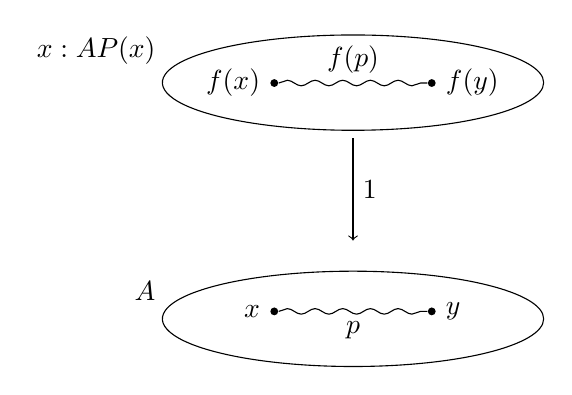
\begin{tikzpicture}[yscale=.5,xscale=2]
\draw (0,0) arc (-90:170:8ex) node[anchor=south east] {$A$} arc (170:270:8ex);
\draw (0,6) arc (-90:170:8ex) node[anchor=south east] {$\sm{x:A} P(x)$} arc (170:270:8ex);
\draw[->] (0,5.8) -- node[auto] {$\proj1$} (0,3.2);
\node[circle,fill,inner sep=1pt,label=left:{$x$}] (b1) at (-.5,1.4) {};
\node[circle,fill,inner sep=1pt,label=right:{$y$}] (b2) at (.5,1.4) {};
\draw[decorate,decoration={snake,amplitude=1}] (b1) -- node[auto,swap] {$p$} (b2);
\node[circle,fill,inner sep=1pt,label=left:{$f(x)$}] (b1) at (-.5,7.2) {};
\node[circle,fill,inner sep=1pt,label=right:{$f(y)$}] (b2) at (.5,7.2) {};
\draw[decorate,decoration={snake,amplitude=1}] (b1) -- node[auto] {$f(p)$} (b2);
\end{tikzpicture}
\end{center}

我们 \emph{可以} 从 \cref{lem:map} 中获得这样的结果。
给定 $f:\prd{x:A} P(x)$,我们可以通过设置 $f'(x)\defeq (x,f(x))$ 来定义一个非依赖函数 $f':A\to \sm{x:A} P(x)$,然后考虑 $\ap{f'}{p} : f'(x) = f'(y)$。
由于 $\proj1 \circ f' \jdeq \idfunc[A]$,通过 \cref{lem:ap-functor} 我们有 $\ap{\proj1}{\ap{f'}{p}} = p$;因此 $\ap{f'}{p}$ 确实在这个意义上“覆盖” $p$。
然而,从 \emph{类型} 的角度来看,$\ap{f'}{p}$ 并不明显覆盖 $A$ 中的任何特定路径(在本例中为 $p$),这在某些情况下可能很重要。

解决方案是使用传递引理。
根据 \cref{thm:path-lifting} 我们有一个从 $(x,u)$ 到 $(y,\trans p u)$ 的规范路径 $\mathsf{lift}(u,p)$,它覆盖 $p$。
因此,任何从 $u:P(x)$ 到 $v:P(y)$ 的路径覆盖 $p$ 应该通过 $\mathsf{lift}(u,p)$ 以基本唯一的方式在 $P(y)$ 的纤维中完全提升。
因此,直到等价性,定义“从 $u$ 到 $v$ 的路径覆盖 $p:x=y$”意义上意味着 $P(y)$ 中的路径 $\trans p u = v$ 是合理的。
而且,事实上,我们可以证明依赖函数会产生这样的路径。

\begin{lem}[依赖映射 (Dependent map)]\label{lem:mapdep}
\indexdef{依赖函数应用于路径 (application!of dependent function to a path)}%
\indexdef{路径!依赖函数应用于路径 (path!application of a dependent function to)}%
\indexdef{函数!依赖!应用于路径 (function!dependent!application to a path of)}%
\indexdef{依赖函数在路径上的作用 (action!of a dependent function on a path)}%
假设 $f:\prd{x: A} P(x)$;那么我们有一个映射
\[\apdfunc f : \prd{p:x=y}\big(\id[P(y)]{\trans p{f(x)}}{f(y)}\big)。\]
\end{lem}

\begin{proof}[第一种证明 (First proof)]
令 $D:\prd{x,y:A} (\id{x}{y}) \to \type$ 为定义为
\begin{equation*}
D(x,y,p)\defeq \trans p {f(x)}= f(y)。
\end{equation*}
的类型族。
然后 $D(x,x,\refl{x})$ 是 $\trans{(\refl{x})}{f(x)}= f(x)$。
但由于 $\trans{(\refl{x})}{f(x)}\jdeq f(x)$,我们得到 $D(x,x,\refl{x})\jdeq (f(x)= f(x))$。
因此,我们找到函数
\begin{equation*}
d\defeq\lam{x} \refl{f(x)}:\prd{x:A} D(x,x,\refl{x})
\end{equation*}
现在路径归纳为每个 $p:x= y$ 给我们 $\apdfunc f(p):\trans p{f(x)}= f(y)$。
\end{proof}

\begin{proof}[第二种证明 (Second proof)]
通过归纳,假设 $p$ 是 $\refl x$ 就足够了。
但在这种情况下,所需的等式是 $\trans{(\refl{x})}{f(x)}= f(x)$,这在判断上是成立的。
\end{proof}

我们通常将这种意义上“覆盖其他路径”的路径称为 \emph{依赖路径 (dependent paths)}。
\indexsee{依赖!路径 (dependent!path)}{路径, 依赖 (path, dependent)}%
\index{路径!依赖 (path!dependent)}%
它们将在 \cref{cha:hits} 中起到越来越重要的作用。
在 \cref{sec:computational} 中我们将看到,对于一些特定类型的类型族,有等价的方法来表示依赖路径的概念,这在某些情况下更为方便。

现在回想一下,在 \cref{sec:pi-types} 中,一个非依赖类型的函数 $f:A\to B$ 只是当 $P$ 是常量类型族 $P(x) \defeq B$ 时的依赖类型函数 $f:\prd{x:A} P(x)$ 的特例。
在这种情况下,$\apdfunc{f}$ 和 $\apfunc{f}$ 是密切相关的,因为有以下引理:

\begin{lem}\label{thm:trans-trivial}
如果 $P:A\to\type$ 定义为 $P(x) \defeq B$ 对于一个固定的 $B:\type$,那么对于任意 $x,y:A$ 和 $p:x=y$ 以及 $b:B$ 我们有路径
\[ \transconst Bpb : \transfib P p b = b。 \]
\end{lem}
\begin{proof}[第一种证明 (First proof)]
固定一个 $b:B$,令 $D:\prd{x,y:A} (\id{x}{y}) \to \type$ 为定义为
\[ D(x,y,p) \defeq (\transfib P p b = b)。\]
的类型族。
然后 $D(x,x,\refl x)$ 是 $(\transfib P{\refl{x}}{b} = b)$,根据传递的计算规则,这在判断上等于 $(b=b)$。
因此,我们有函数
\[ d \defeq \lam{x} \refl{b} : \prd{x:A} D(x,x,\refl x)。\]
现在路径归纳给我们一个
\narrowequation{
\prd{x,y:A}{p:x=y}(\transfib P p b = b),}
的元素,正如我们所希望的那样。
\end{proof}
\begin{proof}[第二种证明 (Second proof)]
通过归纳,假设 $y$ 是 $x$ 并且 $p$ 是 $\refl x$ 就足够了。
但是 $\transfib P {\refl x} b \jdeq b$,因此在这种情况下,我们要证明的是 $b=b$,并且我们有 $\refl{b}$ 可以证明。
\end{proof}

因此,对于任意 $x,y:A$ 和 $p:x=y$ 以及 $f:A\to B$,通过分别与 $\transconst Bp{f(x)}$ 及其逆连接,我们得到函数
\begin{align}
\big(f(x) = f(y)\big) &\to \big(\trans{p}{f(x)} = f(y)\big)\label{eq:ap-to-apd}
\qquad\text{和 (and)} \\
\big(\trans{p}{f(x)} = f(y)\big) &\to \big(f(x) = f(y)\big)。\label{eq:apd-to-ap}
\end{align}
实际上,这些函数是逆等价的(将在 \cref{sec:basics-equivalences} 中介绍),并且它们将 $\apfunc f (p)$ 与 $\apdfunc f (p)$ 关联起来。

\begin{lem}\label{thm:apd-const}
对于 $f:A\to B$ 和 $p:\id[A]xy$,我们有
\[ \apdfunc f(p) = \transconst B p{f(x)} \ct \apfunc f (p)。\]
\end{lem}
\begin{proof}[第一种证明 (First proof)]
令 $D:\prd{x,y:A} (\id xy) \to \type$ 为定义为
\[ D(x,y,p) \defeq \big(\apdfunc f (p) = \transconst Bp{f(x)} \ct \apfunc f (p)\big)。\]
的类型族。
因此,我们有
\[D(x,x,\refl x) \jdeq \big(\apdfunc f (\refl x) = \transconst B{\refl x}{f(x)} \ct \apfunc f ({\refl x})\big)。\]
但根据定义,这三个路径都是 $\refl{f(x)}$,所以我们有
\[ \refl{\refl{f(x)}} : D(x,x,\refl x)。\]
因此,路径归纳为我们提供了 $\prd{x,y:A}{p:x=y} D(x,y,p)$ 的元素,这正是我们想要的。
\end{proof}
\begin{proof}[第二种证明 (Second proof)]
通过归纳,假设 $y$ 是 $x$ 并且 $p$ 是 $\refl x$ 就足够了。
在这种情况下,我们要证明的是 $\refl{f(x)} = \refl{f(x)} \ct \refl{f(x)}$,这是在判断上成立的。
\end{proof}

由于 $\apdfunc{f}$ 和 $\apfunc{f}$ 的类型不同,通常使用不同的符号来表示它们会更清晰。
% 我们有时可能会使用符号 $\apd f p$ 表示 $\apdfunc{f}(p)$,类似于使用符号 $\ap f p$ 表示 $\apfunc{f}(p)$。

\index{函数!依赖 (function!dependent)|)}%

此时,我们希望读者开始熟悉身份类型的归纳证明。
从现在起,我们不再给出两种证明风格,而是允许我们使用最清晰和方便的证明(通常是第二种,更简洁的证明)。
以下是一些关于传递的有用引理;我们将其证明(采用任一风格)留给读者。

\begin{lem}\label{thm:transport-concat}
给定 $P:A\to\type$,其中 $p:\id[A]xy$ 和 $q:\id[A]yz$ 以及 $u:P(x)$,我们有
\[ \trans{q}{\trans{p}{u}} = \trans{(p\ct q)}{u}。 \]
\end{lem}

\begin{lem}\label{thm:transport-compose}
对于函数 $f:A\to B$ 和一个类型族 $P:B\to\type$,以及任意 $p:\id[A]xy$ 和 $u:P(f(x))$,我们有
\[ \transfib{P\circ f}{p}{u} = \transfib{P}{\apfunc f(p)}{u}。 \]
\end{lem}

\begin{lem}\label{thm:ap-transport}
对于 $P,Q:A\to \type$ 和一族函数 $f:\prd{x:A} P(x)\to Q(x)$,以及任意 $p:\id[A]xy$ 和 $u:P(x)$,我们有
\[ \transfib{Q}{p}{f_x(u)} = f_y(\transfib{P}{p}{u})。 \]
\end{lem}

\index{类型!族 (type!family of)|)}%
\index{传递 (transport)|)}

\section{Homotopies and equivalences}
\label{sec:basics-equivalences}

\index{homotopy|(defstyle}%

So far, we have seen how the identity type $\id[A]xy$ can be regarded as a type of \emph{identifications}, \emph{paths}, or \emph{equivalences} between two elements $x$ and~$y$ of a type $A$.
Now we investigate the appropriate notions of ``identification'' or ``sameness'' between \emph{functions} and between \emph{types}.
In \cref{sec:compute-pi,sec:compute-universe}, we will see that homotopy type theory allows us to identify these with instances of the identity type, but before we can do that we need to understand them in their own right.

Traditionally, we regard two functions as the same if they take equal values on all inputs.
Under the propositions-as-types interpretation, this suggests that two functions $f$ and $g$ (perhaps dependently typed) should be the same if the type $\prd{x:A} (f(x)=g(x))$ is inhabited.
Under the homotopical interpretation, this dependent function type consists of \emph{continuous} paths or \emph{functorial} equivalences, and thus may be regarded as the type of \emph{homotopies} or of \emph{natural isomorphisms}.\index{isomorphism!natural}
We will adopt the topological terminology for this.

\begin{defn} \label{defn:homotopy}
  Let $f,g:\prd{x:A} P(x)$ be two sections of a type family $P:A\to\type$.
  A \define{homotopy}
  from $f$ to $g$ is a dependent function of type
  \begin{equation*}
    (f\htpy g) \defeq \prd{x:A} (f(x)=g(x)).
  \end{equation*}
\end{defn}

Note that a homotopy is not the same as an identification $(f=g)$.
However, in \cref{sec:compute-pi} we will introduce an axiom making homotopies and identifications ``equivalent''.

The following proofs are left to the reader.

\begin{lem}\label{lem:homotopy-props}
  Homotopy is an equivalence relation on each dependent function type $\prd{x:A} P(x)$.
  That is, we have elements of the types
  \begin{gather*}
    \prd{f:\prd{x:A} P(x)} (f\htpy f)\\
    \prd{f,g:\prd{x:A} P(x)} (f\htpy g) \to (g\htpy f)\\
    \prd{f,g,h:\prd{x:A} P(x)} (f\htpy g) \to (g\htpy h) \to (f\htpy h).
  \end{gather*}
\end{lem}

% This is judgmental and is \cref{ex:composition}.
% \begin{lem}
%   Composition is associative and unital up to homotopy.
%   That is:
%   \begin{enumerate}
%   \item If $f:A\to B$ then $f\circ \idfunc[A]\htpy f\htpy \idfunc[B]\circ f$.
%   \item If $f:A\to B, g:B\to C$ and $h:C\to D$ then $h\circ (g\circ f) \htpy (h\circ g)\circ f$.
%   \end{enumerate}
% \end{lem}

\index{functoriality of functions in type theory@``functoriality'' of functions in type theory}%
\index{continuity of functions in type theory@``continuity'' of functions in type theory}%
Just as functions in type theory are automatically ``functors'', homotopies are automatically
\index{naturality of homotopies@``naturality'' of homotopies}%
``natural transformations''.
We will state and prove this only for non-dependent functions $f,g:A\to B$; in \cref{ex:dep-htpy-natural} we ask the reader to generalize it to dependent functions.

Recall that for $f:A\to B$ and $p:\id[A]xy$, we may write $\ap f p$ to mean $\apfunc{f} (p)$.

\begin{lem}\label{lem:htpy-natural}
  Suppose $H:f\htpy g$ is a homotopy between functions $f,g:A\to B$ and let $p:\id[A]xy$.  Then we have
  \begin{equation*}
    H(x)\ct\ap{g}{p}=\ap{f}{p}\ct H(y).
  \end{equation*}
  We may also draw this as a commutative diagram:\index{diagram}
  \begin{align*}
    \xymatrix{
      f(x) \ar@{=}[r]^{\ap fp} \ar@{=}[d]_{H(x)} & f(y) \ar@{=}[d]^{H(y)} \\
      g(x) \ar@{=}[r]_{\ap gp} & g(y)
    }
  \end{align*}
\end{lem}
\begin{proof}
  By induction, we may assume $p$ is $\refl x$.
  Since $\apfunc{f}$ and $\apfunc g$ compute on reflexivity, in this case what we must show is
  \[ H(x) \ct \refl{g(x)} = \refl{f(x)} \ct H(x). \]
  But this follows since both sides are equal to $H(x)$.
\end{proof}

\begin{cor}\label{cor:hom-fg}
  Let $H : f \htpy \idfunc[A]$ be a homotopy, with $f : A \to A$. Then for any $x : A$ we have \[ H(f(x)) = \ap f{H(x)}. \]
  % The above path will be denoted by $\com{H}{f}{x}$.
\end{cor}
\noindent
Here $f(x)$ denotes the ordinary application of $f$ to $x$, while $\ap f{H(x)}$ denotes $\apfunc{f}(H(x))$.
\begin{proof}
By naturality of $H$, the following diagram of paths commutes:
\begin{align*}
\xymatrix@C=3pc{
ffx \ar@{=}[r]^-{\ap f{Hx}} \ar@{=}[d]_{H(fx)} & fx \ar@{=}[d]^{Hx} \\
fx \ar@{=}[r]_-{Hx} & x
}
\end{align*}
That is, $\ap f{H x} \ct H x = H(f x) \ct H x$.
We can now whisker by $\opp{(H x)}$ to cancel $H x$, obtaining
\[ \ap f{H x}
= \ap f{H x} \ct H x \ct \opp{(H x)}
= H(f x) \ct H x \ct \opp{(H x)}
= H(f x)
\]
as desired (with some associativity paths suppressed).
\end{proof}

Of course, like the functoriality of functions (\cref{lem:ap-functor}), the equality in \cref{lem:htpy-natural} is a path which satisfies its own coherence laws, and so on.

\index{homotopy|)}%

\index{equivalence|(}%
Moving on to types, from a traditional perspective one may say that a function $f:A\to B$ is an \emph{isomorphism} if there is a function $g:B\to A$ such that both composites $f\circ g$ and $g\circ f$ are pointwise equal to the identity, i.e.\ such that $f \circ g \htpy \idfunc[B]$ and $g\circ f \htpy \idfunc[A]$.
\indexsee{homotopy!equivalence}{equivalence}%
A homotopical perspective suggests that this should be called a \emph{homotopy equivalence}, and from a categorical one, it should be called an \emph{equivalence of (higher) groupoids}.
However, when doing proof-relevant mathematics,
\index{mathematics!proof-relevant}%
the corresponding type
\begin{equation}
  \sm{g:B\to A} \big((f \circ g \htpy \idfunc[B]) \times (g\circ f \htpy \idfunc[A])\big)\label{eq:qinvtype}
\end{equation}
is poorly behaved.
For instance, for a single function $f:A\to B$ there may be multiple unequal inhabitants of~\eqref{eq:qinvtype}.
(This is closely related to the observation in higher category theory that often one needs to consider \emph{adjoint} equivalences\index{adjoint!equivalence} rather than plain equivalences.)
For this reason, we give~\eqref{eq:qinvtype} the following historically accurate, but slightly de\-rog\-a\-to\-ry-sounding name instead.

\begin{defn}\label{defn:quasi-inverse}
  For a function $f:A\to B$, a \define{quasi-inverse}
  \indexdef{quasi-inverse}%
  \indexsee{function!quasi-inverse of}{quasi-inverse}%
  of $f$ is a triple $(g,\alpha,\beta)$ consisting of a function $g:B\to A$ and homotopies
$\alpha:f\circ g\htpy \idfunc[B]$ and $\beta:g\circ f\htpy \idfunc[A]$.
\end{defn}

\symlabel{qinv}
Thus,~\eqref{eq:qinvtype} is \emph{the type of quasi-inverses of $f$}; we may denote it by $\qinv(f)$.

\begin{eg}\label{eg:idequiv}
  \index{identity!function}%
  \index{function!identity}%
  The identity function $\idfunc[A]:A\to A$ has a quasi-inverse given by $\idfunc[A]$ itself, together with homotopies defined by $\alpha(y) \defeq \refl{y}$ and $\beta(x) \defeq \refl{x}$.
\end{eg}

\begin{eg}\label{eg:concatequiv}
  For any $p:\id[A]xy$ and $z:A$, the functions
  \begin{align*}
    (p\ct \blank)&:(\id[A]yz) \to (\id[A]xz) \qquad\text{and}\\
    (\blank \ct p)&:(\id[A]zx) \to (\id[A]zy)
  \end{align*}
  have quasi-inverses given by $(\opp p \ct \blank)$ and $(\blank \ct \opp p)$, respectively; see \cref{ex:equiv-concat}.
\end{eg}

\begin{eg}\label{thm:transportequiv}
  For any $p:\id[A]xy$ and $P:A\to\type$, the function
  \[\transfib{P}{p}{\blank}:P(x) \to P(y)\]
  has a quasi-inverse given by $\transfib{P}{\opp p}{\blank}$; this follows from \narrowbreak \cref{thm:transport-concat}.
\end{eg}

\symlabel{basics-isequiv}\symlabel{basics:iso}
In general, we will only use the word \emph{isomorphism}
\index{isomorphism!of sets}
(and similar words such as \emph{bijection}, and the associated notation $A\cong B$)
\index{bijection}
in the special case when the types $A$ and $B$ ``behave like sets'' (see \cref{sec:basics-sets}).
In this case, the type~\eqref{eq:qinvtype} is unproblematic.
We will reserve the word \emph{equivalence} for an improved notion $\isequiv (f)$ with the following properties:%
\begin{enumerate}
\item For each $f:A\to B$ there is a function $\qinv(f) \to \isequiv (f)$.\label{item:be1}
\item Similarly, for each $f$ we have $\isequiv (f) \to \qinv(f)$; thus the two are logically equivalent (see \cref{sec:pat}).\label{item:be2}
\item For any two inhabitants $e_1,e_2:\isequiv(f)$ we have $e_1=e_2$.\label{item:be3}
\end{enumerate}
In \cref{cha:equivalences} we will see that there are many different definitions of $\isequiv(f)$ which satisfy these three properties, but that all of them are equivalent.
For now, to convince the reader that such things exist, we mention only the easiest such definition:
\begin{equation}\label{eq:isequiv-invertible}
  \isequiv(f) \;\defeq\;
  \Parens{\sm{g:B\to A} (f\circ g \htpy \idfunc[B])}
  \times
  \Parens{\sm{h:B\to A} (h\circ f \htpy \idfunc[A])}.
\end{equation}
We can show~\ref{item:be1} and~\ref{item:be2} for this definition now.
A function $\qinv(f) \to \isequiv (f)$ is easy to define by taking $(g,\alpha,\beta)$ to $(g,\alpha,g,\beta)$.
In the other direction, given $(g,\alpha,h,\beta)$, let $\gamma$ be the composite homotopy
\[ g \overset{\beta}{\htpy} h\circ f\circ g \overset{\alpha}{\htpy} h, \]
meaning that $\gamma(x) \defeq \opp{\beta(g(x))} \ct \ap{h}{\alpha(x)}$.
Now define $\beta':g\circ f\htpy \idfunc[A]$ by $\beta'(x) \defeq \gamma(f(x)) \ct \beta(x)$.
Then $(g,\alpha,\beta'):\qinv(f)$.

Property~\ref{item:be3} for this definition is not too hard to prove either, but it requires identifying the identity types of cartesian products and dependent pair types, which we will discuss in \cref{sec:compute-cartprod,sec:compute-sigma}.
Thus, we postpone it as well; see \cref{sec:biinv}.
At this point, the main thing to take away is that there is a well-behaved type which we can pronounce as ``$f$ is an equivalence'', and that we can prove $f$ to be an equivalence by exhibiting a quasi-inverse to it.
In practice, this is the most common way to prove that a function is an equivalence.

In accord with the proof-relevant philosophy,
\index{mathematics!proof-relevant}%
\emph{an equivalence} from $A$ to $B$ is defined to be a function $f:A\to B$ together with an inhabitant of $\isequiv (f)$, i.e.\ a proof that it is an equivalence.
We write $(\eqv A B)$ for the type of equivalences from $A$ to $B$, i.e.\ the type
\begin{equation}\label{eq:eqv}
  (\eqv A B) \defeq \sm{f:A\to B} \isequiv(f).
\end{equation}
Property~\ref{item:be3} above will ensure that if two equivalences are equal as functions (that is, the underlying elements of $A\to B$ are equal), then they are also equal as equivalences (see \cref{sec:compute-sigma}).
Thus, we often abuse notation and blur the distinction between equivalences and their underlying functions.
For instance, if we have a function $f:A\to B$ and we know that $e:\isequiv(f)$, we may write $f:\eqv A B$, rather than $\tup{f}{e}$.
Or conversely, if we have an equivalence $g:\eqv A B$, we may write $g(a)$ when given $a:A$, rather than $(\proj1 g)(a)$.

We conclude by observing:

\begin{lem}\label{thm:equiv-eqrel}
  Type equivalence is an equivalence relation on \type.
  More specifically:
  \begin{enumerate}
  \item For any $A$, the identity function $\idfunc[A]$ is an equivalence; hence $\eqv A A$.
  \item For any $f:\eqv A B$, we have an equivalence $f^{-1} : \eqv B A$.
  \item For any $f:\eqv A B$ and $g:\eqv B C$, we have $g\circ f : \eqv A C$.
  \end{enumerate}
\end{lem}
\begin{proof}
  The identity function is clearly its own quasi-inverse; hence it is an equivalence.

  If $f:A\to B$ is an equivalence, then it has a quasi-inverse, say $f^{-1}:B\to A$.
  Then $f$ is also a quasi-inverse of $f^{-1}$, so $f^{-1}$ is an equivalence $B\to A$.

  Finally, given $f:\eqv A B$ and $g:\eqv B C$ with quasi-inverses $f^{-1}$ and $g^{-1}$, say, then for any $a:A$ we have $f^{-1} g^{-1} g f a = f^{-1} f a = a$, and for any $c:C$ we have $g f f^{-1} g^{-1} c = g g^{-1} c = c$.
  Thus $f^{-1} \circ g^{-1}$ is a quasi-inverse to $g\circ f$, hence the latter is an equivalence.
\end{proof}

\index{equivalence|)}%


\section{The higher groupoid structure of type formers}
\label{sec:computational}

In \cref{cha:typetheory}, we introduced many ways to form new types: cartesian products, disjoint unions, dependent products, dependent sums, etc.
In \cref{sec:equality,sec:functors,sec:fibrations}, we saw that \emph{all} types in homotopy type theory behave like spaces or higher groupoids.
Our goal in the rest of the chapter is to make explicit how this higher structure behaves in the case of the particular types defined in \cref{cha:typetheory}.

It turns out that for many types $A$, the equality types $\id[A]xy$ can be characterized, up to equivalence, in terms of whatever data was used to construct $A$.
For example, if $A$ is a cartesian product $B\times C$, and $x\jdeq (b,c)$ and $y\jdeq(b',c')$, then we have an equivalence
\begin{equation}\label{eq:prodeqv}
  \eqv{\big((b,c)=(b',c')\big)}{\big((b=b')\times (c=c')\big)}.
\end{equation}
In more traditional language, two ordered pairs are equal just when their components are equal (but the equivalence~\eqref{eq:prodeqv} says rather more than this).
The higher structure of the identity types can also be expressed in terms of these equivalences; for instance, concatenating two equalities between pairs corresponds to pairwise concatenation.

Similarly, when a type family $P:A\to\type$ is built up fiberwise using the type forming rules from \cref{cha:typetheory}, the operation $\transfib{P}{p}{\blank}$ can be characterized, up to homotopy, in terms of the corresponding operations on the data that went into $P$.
For instance, if $P(x) \jdeq B(x)\times C(x)$, then we have
\[\transfib{P}{p}{(b,c)} = \big(\transfib{B}{p}{b},\transfib{C}{p}{c}\big).\]

Finally, the type forming rules are also functorial, and if a function $f$ is built from this functoriality, then the operations $\apfunc f$ and $\apdfunc f$ can be computed based on the corresponding ones on the data going into $f$.
For instance, if $g:B\to B'$ and $h:C\to C'$ and we define $f:B\times C \to B'\times C'$ by $f(b,c)\defeq (g(b),h(c))$, then modulo the equivalence~\eqref{eq:prodeqv}, we can identify $\apfunc f$ with ``$(\apfunc g,\apfunc h)$''.

The next few sections (\crefrange{sec:compute-cartprod}{sec:compute-nat}) will be devoted to stating and proving theorems of this sort for all the basic type forming rules, with one section for each basic type former.
Here we encounter a certain apparent deficiency in currently available type theories;
as will become clear in later chapters, it would seem to be more convenient and intuitive if these characterizations of identity types, transport, and so on were \emph{judgmental}\index{judgmental equality} equalities.
However, in the theory presented in \cref{cha:typetheory}, the identity types are defined uniformly for all types by their induction principle, so we cannot ``redefine'' them to be different things at different types.
Thus, the characterizations for particular types to be discussed in this chapter are, for the most part, \emph{theorems} which we have to discover and prove, if possible.

Actually, the type theory of \cref{cha:typetheory} is insufficient to prove the desired theorems for two of the type formers: $\Pi$-types and universes.
For this reason, we are forced to introduce axioms into our type theory, in order to make those ``theorems'' true.
Type-theoretically, an \emph{axiom} (c.f.~\cref{sec:axioms}) is an ``atomic'' element that is declared to inhabit some specified type, without there being any rules governing its behavior other than those pertaining to the type it inhabits.
\index{axiom!versus rules}%

\index{function extensionality}%
\indexsee{extensionality, of functions}{function extensionality}
\index{univalence axiom}%
The axiom for $\Pi$-types (\cref{sec:compute-pi}) is familiar to type theorists: it is called \emph{function extensionality}, and states (roughly) that if two functions are homotopic in the sense of \cref{sec:basics-equivalences}, then they are equal.
The axiom for universes (\cref{sec:compute-universe}), however, is a new contribution of homotopy type theory due to Voevodsky: it is called the \emph{univalence axiom}, and states (roughly) that if two types are equivalent in the sense of \cref{sec:basics-equivalences}, then they are equal.
We have already remarked on this axiom in the introduction; it will play a very important role in this book.%
\footnote{We have chosen to introduce these principles as axioms, but there are potentially other ways to formulate a type theory in which they hold.
  See the Notes to this chapter.}

It is important to note that not \emph{all} identity types can be ``determined'' by induction over the construction of types.
Counterexamples include most nontrivial higher inductive types (see \cref{cha:hits,cha:homotopy}).
For instance, calculating the identity types of the types $\Sn^n$ (see \cref{sec:circle}) is equivalent to calculating the higher homotopy groups of spheres, a deep and important field of research in algebraic topology.


\section{Cartesian product types}
\label{sec:compute-cartprod}

\index{type!product|(}%
Given types $A$ and $B$, consider the cartesian product type $A \times B$.
For any elements $x,y:A\times B$ and a path $p:\id[A\times B]{x}{y}$, by functoriality we can extract paths $\ap{\proj1}p:\id[A]{\proj1(x)}{\proj1(y)}$ and $\ap{\proj2}p:\id[B]{\proj2(x)}{\proj2(y)}$.
Thus, we have a function
\begin{equation}\label{eq:path-prod}
  (\id[A\times B]{x}{y}) \to (\id[A]{\proj1(x)}{\proj1(y)}) \times (\id[B]{\proj2(x)}{\proj2(y)}).
\end{equation}

\begin{thm}\label{thm:path-prod}
  For any $x$ and $y$, the function~\eqref{eq:path-prod} is an equivalence.
\end{thm}

Read logically, this says that two pairs are equal just if they are equal
componentwise.  Read category-theoretically, this says that the
morphisms in a product groupoid are pairs of morphisms.  Read
homotopy-theoretically, this says that the paths in a product
space are pairs of paths.

\begin{proof}
  We need a function in the other direction:
  \begin{equation}
    (\id[A]{\proj1(x)}{\proj1(y)}) \times (\id[B]{\proj2(x)}{\proj2(y)}) \to (\id[A\times B]{x}{y}). \label{eq:path-prod-inverse}
  \end{equation}
  By the induction rule for cartesian products, we may assume that $x$ and $y$ are both pairs, i.e.\ $x\jdeq (a,b)$ and $y\jdeq (a',b')$ for some $a,a':A$ and $b,b':B$.
  In this case, what we want is a function
  \begin{equation*}
    (\id[A]{a}{a'}) \times (\id[B]{b}{b'}) \to \big(\id[A\times B]{(a,b)}{(a',b')}\big).
  \end{equation*}
  Now by induction for the cartesian product in its domain, we may assume given $p:a=a'$ and $q:b=b'$.
  And by two path inductions, we may assume that $a\jdeq a'$ and $b\jdeq b'$ and both $p$ and $q$ are reflexivity.
  But in this case, we have $(a,b)\jdeq(a',b')$ and so we can take the output to also be reflexivity.

  It remains to prove that~\eqref{eq:path-prod-inverse} is quasi-inverse to~\eqref{eq:path-prod}.
  This is a simple sequence of inductions, but they have to be done in the right order.

  In one direction, let us start with $r:\id[A\times B]{x}{y}$.
  We first do a path induction on $r$ in order to assume that $x\jdeq y$ and $r$ is reflexivity.
  In this case, since $\apfunc{\proj1}$ and $\apfunc{\proj2}$ are defined by path induction,~\eqref{eq:path-prod} takes $r\jdeq \refl{x}$ to the pair $(\refl{\proj1x},\refl{\proj2x})$.
  Now by induction on $x$, we may assume $x\jdeq (a,b)$, so that this is $(\refl a, \refl b)$.
  Thus,~\eqref{eq:path-prod-inverse} takes it by definition to $\refl{(a,b)}$, which (under our current assumptions) is $r$.

  In the other direction, if we start with $s:(\id[A]{\proj1(x)}{\proj1(y)}) \times (\id[B]{\proj2(x)}{\proj2(y)})$, then we first do induction on $x$ and $y$ to assume that they are pairs $(a,b)$ and $(a',b')$, and then induction on $s:(\id[A]{a}{a'}) \times (\id[B]{b}{b'})$ to reduce it to a pair $(p,q)$ where $p:a=a'$ and $q:b=b'$.
  Now by induction on $p$ and $q$, we may assume they are reflexivities $\refl a$ and $\refl b$, in which case~\eqref{eq:path-prod-inverse} yields $\refl{(a,b)}$ and then~\eqref{eq:path-prod} returns us to $(\refl a,\refl b)\jdeq (p,q)\jdeq s$.
\end{proof}

In particular, we have shown that~\eqref{eq:path-prod} has an inverse~\eqref{eq:path-prod-inverse}, which we may denote by
\symlabel{defn:pairpath}
\[
\pairpath : (\id{\proj{1}(x)}{\proj{1}(y)}) \times (\id{\proj{2}(x)}{\proj{2}(y)}) \to (\id x y).
\]
Note that a special case of this yields the propositional uniqueness principle\index{uniqueness!principle, propositional!for product types} for products: $z = (\proj1(z),\proj2(z))$.

It can be helpful to view \pairpath as a \emph{constructor} or \emph{introduction rule} for $\id x y$, analogous to the ``pairing'' constructor of $A\times B$ itself, which introduces the pair $(a,b)$ given $a:A$ and $b:B$.
From this perspective, the two components of~\eqref{eq:path-prod}:
\begin{align*}
  \projpath{1} &: (\id{x}{y}) \to (\id{\proj{1}(x)}{\proj{1} (y)})\\
  \projpath{2} &: (\id{x}{y}) \to (\id{\proj{2}(x)}{\proj{2} (y)})
\end{align*}
are \emph{elimination} rules.
Similarly, the two homotopies which witness~\eqref{eq:path-prod-inverse} as quasi-inverse to~\eqref{eq:path-prod} consist, respectively, of \emph{propositional computation rules}:
\index{computation rule!propositional!for identities between pairs}%
\begin{align*}
  {\projpath{1}{(\pairpath(p, q)})}
  &= %_{(\id{\proj{1} x}{\proj{1} y})}
  {p} \\
  {\projpath{2}{(\pairpath(p,q)})}
  &= %_{(\id{\proj{2} x}{\proj{2} y})}
  {q}
\end{align*}
for $p:\id{\proj{1} x}{\proj{1} y}$ and $q:\id{\proj{2} x}{\proj{2} y}$,
and a \emph{propositional uniqueness principle}:
\index{uniqueness!principle, propositional!for identities between pairs}%
\[
\id{r}{\pairpath(\projpath{1} (r), \projpath{2} (r)) }
\qquad\text{for } r : \id[A \times B] x y.
\]

We can also characterize the reflexivity, inverses, and composition of paths in $A\times B$ componentwise:
\begin{align*}
  {\refl{(z : A \times B)}}
  &= {\pairpath (\refl{\proj{1} z},\refl{\proj{2} z})} \\
  {\opp{p}}
  &= {\pairpath \big(\opp{\projpath{1} (p)},\, \opp{\projpath{2} (p)}\big)} \\
  {{p \ct q}}
  &= {\pairpath \big({\projpath{1} (p)} \ct {\projpath{1} (q)},\,{\projpath{2} (p)} \ct {\projpath{2} (q)}\big)}.
\end{align*}
Or, written differently:
\begin{alignat*}{2}
  \projpath{i}(\refl{(z : A \times B)}) &= \refl{\proj{i} z} &\qquad (i=1,2)\\
  \pairpath(\opp p, \opp q) &= \opp{\pairpath(p,q)}\\
  \pairpath(p\ct q, p'\ct q') &= \pairpath(p,p') \ct \pairpath(q,q').
\end{alignat*}
All of these equations can be derived by using path induction on the given paths and then returning reflexivity.
The same is true for the rest of the higher groupoid structure considered in \cref{sec:equality}, although it begins to get tedious to insert enough other coherence paths to yield an equation that will typecheck.
For instance, if we denote the inverse of the path in \cref{thm:omg}\ref{item:omg4} by $\ctassoc(p,q,r)$ and the last path displayed above by $\pairct(p,q,p',q')$, then for any $u,v,z,w:A\times B$ and $p,q,r,p',q',r'$ of appropriate types we have
\begin{equation*}
  \begin{array}{l}
    \pairct(p\ct q, r, p'\ct q', r') \\
    \ct\;  (\pairct(p,q,p',q') \rightwhisker \pairpath(r,r')) \\
    \ct\;  \ctassoc(\pairpath(p,p'),\pairpath(q,q'),\pairpath(r,r'))\\
    =
    \begin{array}[t]{l}
      \apfunc{\pairpath}({\pairpath(\ctassoc(p,q,r),\ctassoc(p',q',r'))})\\
      \ct\; \pairct(p, q\ct r, p', q'\ct r')\\
      \ct\; (\pairpath(p,p') \leftwhisker \pairct(q,r,q',r')).
    \end{array}
  \end{array}
\end{equation*}
Fortunately, we will never have to use any such higher-dimensional coherences.

\index{transport!in product types}%
We now consider transport in a pointwise product of type families.
Given type families $ A, B : Z \to \type$, we abusively write $A\times B:Z\to \type$ for the type family defined by $(A\times B)(z) \defeq A(z) \times B(z)$.
Now given $p : \id[Z]{z}{w}$ and $x : A(z) \times B(z)$, we can transport $x$ along $p$ to obtain an element of $A(w)\times B(w)$.

\begin{thm}\label{thm:trans-prod}
  In the above situation, we have
  \[
  \id[A(w) \times B(w)]
  {\transfib{A\times B}px}
  {(\transfib{A}{p}{\proj{1}x}, \transfib{B}{p}{\proj{2}x})}.
  \]
\end{thm}
\begin{proof}
  By path induction, we may assume $p$ is reflexivity, in which case we have
  \begin{align*}
    \transfib{A\times B}px&\jdeq x\\
    \transfib{A}{p}{\proj{1}x}&\jdeq \proj1x\\
    \transfib{B}{p}{\proj{2}x}&\jdeq \proj2x.
  \end{align*}
  Thus, it remains to show $x = (\proj1 x, \proj2x)$.
  But this is the propositional uniqueness principle for product types, which, as we remarked above, follows from \cref{thm:path-prod}.
\end{proof}

Finally, we consider the functoriality of $\apfunc{}$ under cartesian products.
Suppose given types $A,B,A',B'$ and functions $g:A\to A'$ and $h:B\to B'$; then we can define a function $f:A\times B\to A'\times B'$ by $f(x) \defeq (g(\proj1x),h(\proj2x))$.

\begin{thm}\label{thm:ap-prod}
  In the above situation, given $x,y:A\times B$ and $p:\proj1x=\proj1y$ and $q:\proj2x=\proj2y$, we have
  \[ \id[(f(x)=f(y))]{\ap{f}{\pairpath(p,q)}} {\pairpath(\ap{g}{p},\ap{h}{q})}. \]
\end{thm}
\begin{proof}
  Note first that the above equation is well-typed.
  On the one hand, since $\pairpath(p,q):x=y$ we have $\ap{f}{\pairpath(p,q)}:f(x)=f(y)$.
  On the other hand, since $\proj1(f(x))\jdeq g(\proj1x)$ and $\proj2(f(x))\jdeq h(\proj2x)$, we also have $\pairpath(\ap{g}{p},\ap{h}{q}):f(x)=f(y)$.

  Now, by induction, we may assume $x\jdeq(a,b)$ and $y\jdeq(a',b')$, in which case we have $p:a=a'$ and $q:b=b'$.
  Thus, by path induction, we may assume $p$ and $q$ are reflexivity, in which case the desired equation holds judgmentally.
\end{proof}

\index{type!product|)}%

\section{\texorpdfstring{$\Sigma$}{Σ}-types}
\label{sec:compute-sigma}

\index{type!dependent pair|(}%
Let $A$ be a type and $P:A\to\type$ a type family.
Recall that the $\Sigma$-type, or dependent pair type, $\sm{x:A} P(x)$ is a generalization of the cartesian product type.
Thus, we expect its higher groupoid structure to also be a generalization of the previous section.
In particular, its paths should be pairs of paths, but it takes a little thought to give the correct types of these paths.

Suppose that we have a path $p:w=w'$ in $\sm{x:A}P(x)$.
Then we get $\ap{\proj{1}}{p}:\proj{1}(w)=\proj{1}(w')$.
However, we cannot directly ask whether $\proj{2}(w)$ is identical to $\proj{2}(w')$ since they don't have to be in the same type.
But we can transport\index{transport} $\proj{2}(w)$ along the path $\ap{\proj{1}}{p}$, and this does give us an element of the same type as $\proj{2}(w')$.
By path induction, we do in fact obtain a path $\trans{\ap{\proj{1}}{p}}{\proj{2}(w)}=\proj{2}(w')$.

Recall from the discussion preceding \cref{lem:mapdep} that
\narrowequation{
  \trans{\ap{\proj{1}}{p}}{\proj{2}(w)}=\proj{2}(w')
}
can be regarded as the type of paths from $\proj2(w)$ to $\proj2(w')$ which lie over the path $\ap{\proj1}{p}$ in $A$.
\index{fibration}%
\index{total!space}%
Thus, we are saying that a path $w=w'$ in the total space determines (and is determined by) a path $p:\proj1(w)=\proj1(w')$ in $A$ together with a path from $\proj2(w)$ to $\proj2(w')$ lying over $p$, which seems sensible.

\begin{rmk}
  Note that if we have $x:A$ and $u,v:P(x)$ such that $(x,u)=(x,v)$, it does not follow that $u=v$.
  All we can conclude is that there exists $p:x=x$ such that $\trans p u = v$.
  This is a well-known source of confusion for newcomers to type theory, but it makes sense from a topological viewpoint: the existence of a path $(x,u)=(x,v)$ in the total space of a fibration between two points that happen to lie in the same fiber does not imply the existence of a path $u=v$ lying entirely \emph{within} that fiber.
\end{rmk}

The next theorem states that we can also reverse this process.
Since it is a direct generalization of \cref{thm:path-prod}, we will be more concise.

\begin{thm}\label{thm:path-sigma}
Suppose that $P:A\to\type$ is a type family over a type $A$ and let $w,w':\sm{x:A}P(x)$. Then there is an equivalence
\begin{equation*}
\eqvspaced{(w=w')}{\dsm{p:\proj{1}(w)=\proj{1}(w')} \trans{p}{\proj{2}(w)}=\proj{2}(w')}.
\end{equation*}
\end{thm}

\begin{proof}
We define a function
\begin{equation*}
f : \prd{w,w':\sm{x:A}P(x)} (w=w') \to \dsm{p:\proj{1}(w)=\proj{1}(w')} \trans{p}{\proj{2}(w)}=\proj{2}(w')
\end{equation*}
by path induction, with
\begin{equation*}
f(w,w,\refl{w})\defeq(\refl{\proj{1}(w)},\refl{\proj{2}(w)}).
\end{equation*}
We want to show that $f$ is an equivalence.

In the reverse direction, we define
\begin{narrowmultline*}
  g : \prd{w,w':\sm{x:A}P(x)}
      \Parens{\sm{p:\proj{1}(w)=\proj{1}(w')}\trans{p}{\proj{2}(w)}=\proj{2}(w')}
      \to
      \narrowbreak
      (w=w')
\end{narrowmultline*}
by first inducting on $w$ and $w'$, which splits them into $(w_1,w_2)$ and
$(w_1',w_2')$ respectively, so it suffices to show
\begin{equation*}
\Parens{\sm{p:w_1 = w_1'}\trans{p}{w_2}=w_2'} \to ((w_1,w_2)=(w_1',w_2')).
\end{equation*}
Next, given a pair $\sm{p:w_1 = w_1'}\trans{p}{w_2}=w_2'$, we can
use $\Sigma$-induction to get $p : w_1 = w_1'$ and $q :
\trans{p}{w_2}=w_2'$.  Inducting on $p$, we have $q :
\trans{(\refl{w_1})}{w_2}=w_2'$, and it suffices to show
$(w_1,w_2)=(w_1,w_2')$.  But $\trans{(\refl{w_1})}{w_2} \jdeq w_2$, so
inducting on $q$ reduces the goal to
$(w_1,w_2)=(w_1,w_2)$, which we can prove with $\refl{(w_1,w_2)}$.

Next we show that $f(g(r))=r$ for all $w$, $w'$ and
$r$, where $r$ has type
\[\dsm{p:\proj{1}(w)=\proj{1}(w')} (\trans{p}{\proj{2}(w)}=\proj{2}(w')).\]
First, we break apart the pairs $w$, $w'$, and $r$ by pair induction, as in the
definition of $g$, and then use two path inductions to reduce both components
of $r$ to \refl{}.  Then it suffices to show that
$f (g(\refl{w_1},\refl{w_2})) = (\refl{w_1},\refl{w_2})$, which is true by definition.

Similarly, to show that $g(f(p))=p$ for all $w$, $w'$,
and $p : w = w'$, we can do path induction on $p$, and then pair induction to
split $w$, at which point it suffices to show that
$g(f (\refl{(w_1,w_2)})) = \refl{(w_1,w_2)}$, which is true by
definition.

Thus, $f$ has a quasi-inverse, and is therefore an equivalence.
\end{proof}

As we did in the case of cartesian products, we can deduce a propositional uniqueness principle as a special case.

\begin{cor}\label{thm:eta-sigma}
  \index{uniqueness!principle, propositional!for dependent pair types}%
  For $z:\sm{x:A} P(x)$, we have $z = (\proj1(z),\proj2(z))$.
\end{cor}
\begin{proof}
  We have $\refl{\proj1(z)} : \proj1(z) = \proj1(\proj1(z),\proj2(z))$, so by \cref{thm:path-sigma} it will suffice to exhibit a path $\trans{(\refl{\proj1(z)})}{\proj2(z)} = \proj2(\proj1(z),\proj2(z))$.
  But both sides are judgmentally equal to $\proj2(z)$.
\end{proof}

Like with binary cartesian products, we can think of
the backward direction of \cref{thm:path-sigma} as
an introduction form (\pairpath{}{}), the forward direction as
elimination forms (\projpath{1} and \projpath{2}), and the equivalence
as giving a propositional computation rule and uniqueness principle for these.

Note that the lifted path $\mathsf{lift}(u,p)$  of $p:x=y$ at $u:P(x)$ defined in \cref{thm:path-lifting} may be identified with the special case of the introduction form
\[\pairpath(p,\refl{\trans p u}):(x,u) = (y,\trans p u).\]
\index{transport!in dependent pair types}%
This appears in the statement of action of transport on $\Sigma$-types, which is also a generalization of the action for binary cartesian products:

\begin{thm}\label{transport-Sigma}
  Suppose we have type families
  %
  \begin{equation*}
    P:A\to\type
    \qquad\text{and}\qquad
    Q:\Parens{\sm{x:A} P(x)}\to\type.
  \end{equation*}
  %
  Then we can construct the type family over $A$ defined by
  \begin{equation*}
    x \mapsto \sm{u:P(x)} Q(x,u).
  \end{equation*}
  For any path $p:x=y$ and any $(u,z):\sm{u:P(x)} Q(x,u)$ we have
  \begin{equation*}
    \trans{p}{u,z}=\big(\trans{p}{u},\,\trans{\pairpath(p,\refl{\trans pu})}{z}\big).
  \end{equation*}
\end{thm}

\begin{proof}
Immediate by path induction.
\end{proof}

We leave it to the reader to state and prove a generalization of
\cref{thm:ap-prod} (see \cref{ex:ap-sigma}), and to characterize
the reflexivity, inverses, and composition of $\Sigma$-types
componentwise.

\index{type!dependent pair|)}%

\section{The unit type}
\label{sec:compute-unit}

\index{type!unit|(}%
Trivial cases are sometimes important, so we mention briefly the case of the unit type~\unit.

\begin{thm}\label{thm:path-unit}
  For any $x,y:\unit$, we have $\eqv{(x=y)}{\unit}$.
\end{thm}

It may be tempting to begin this proof by $\unit$-induction on $x$ and $y$, reducing the problem to $\eqv{(\ttt=\ttt)}{\unit}$.
However, at this point we would be stuck, since we would be unable to perform a path induction on $p:\ttt=\ttt$.
Thus, we instead work with a general $x$ and $y$ as much as possible, reducing them to $\ttt$ by induction only at the last moment.

\begin{proof}
  A function $(x=y)\to\unit$ is easy to define by sending everything to \ttt.
  Conversely, for any $x,y:\unit$ we may assume by induction that $x\jdeq \ttt\jdeq y$.
  In this case we have $\refl{\ttt}:x=y$, yielding a constant function $\unit\to(x=y)$.

  To show that these are inverses, consider first an element $u:\unit$.
  We may assume that $u\jdeq\ttt$, but this is also the result of the composite $\unit \to (x=y)\to\unit$.

  On the other hand, suppose given $p:x=y$.
  By path induction, we may assume $x\jdeq y$ and $p$ is $\refl x$.
  We may then assume that $x$ is \ttt, in which case the composite $(x=y) \to \unit\to(x=y)$ takes $p$ to $\refl x$, i.e.\ to~$p$.
\end{proof}

In particular, any two elements of $\unit$ are equal.
We leave it to the reader to formulate this equivalence in terms of introduction, elimination, computation, and uniqueness rules.
\index{transport!in unit type}%
The transport lemma for \unit is simply the transport lemma for constant type families (\cref{thm:trans-trivial}).

\index{type!unit|)}%

\section{\texorpdfstring{$\Pi$}{Π}-types and the function extensionality axiom}
\label{sec:compute-pi}

\index{type!dependent function|(}%
\index{type!function|(}%
\index{homotopy|(}%
Given a type $A$ and a type family $B : A \to \type$, consider the dependent function type $\prd{x:A}B(x)$.
We expect the type $f=g$ of paths from $f$ to $g$ in $\prd{x:A} B(x)$ to be equivalent to
the type of pointwise paths:\index{pointwise!equality of functions}
\begin{equation}
  \eqvspaced{(\id{f}{g})}{\Parens{\prd{x:A} (\id[B(x)]{f(x)}{g(x)})}}.\label{eq:path-forall}
\end{equation}
From a traditional perspective, this would say that two functions which are equal at each point are equal as functions.
\index{continuity of functions in type theory@``continuity'' of functions in type theory}%
From a topological perspective, it would say that a path in a function space is the same as a continuous homotopy.
\index{functoriality of functions in type theory@``functoriality'' of functions in type theory}%
And from a categorical perspective, it would say that an isomorphism in a functor category is a natural family of isomorphisms.

Unlike the case in the previous sections, however, the basic type theory presented in \cref{cha:typetheory} is insufficient to prove~\eqref{eq:path-forall}.
All we can say is that there is a certain function
\begin{equation}\label{eq:happly}
  \happly : (\id{f}{g}) \to \prd{x:A} (\id[B(x)]{f(x)}{g(x)})
\end{equation}
which is easily defined by path induction.
For the moment, therefore, we will assume:

\begin{axiom}[Function extensionality]\label{axiom:funext}
  \indexsee{axiom!function extensionality}{function extensionality}%
  \indexdef{function extensionality}%
  For any $A$, $B$, $f$, and $g$, the function~\eqref{eq:happly} is an equivalence.
\end{axiom}

We will see in later chapters that this axiom follows both from univalence (see \cref{sec:compute-universe,sec:univalence-implies-funext}) and from an interval type (see \cref{sec:interval} and \cref{ex:funext-from-interval}).

In particular, \cref{axiom:funext} implies that~\eqref{eq:happly} has a quasi-inverse
\[
\funext : \Parens{\prd{x:A} (\id{f(x)}{g(x)})} \to {(\id{f}{g})}.
\]
This function is also referred to as ``function extensionality''.
As we did with $\pairpath$ in \cref{sec:compute-cartprod}, we can regard $\funext$ as an \emph{introduction rule} for the type $\id f g$.
From this point of view, $\happly$ is the \emph{elimination rule}, while the homotopies witnessing $\funext$ as quasi-inverse to $\happly$ become a propositional computation rule\index{computation rule!propositional!for identities between functions}
\[
\id{\happly({\funext{(h)}},x)}{h(x)} \qquad\text{for }h:\prd{x:A} (\id{f(x)}{g(x)})
\]
and a propositional uniqueness principle\index{uniqueness!principle!for identities between functions}:
\[
\id{p}{\funext (x \mapsto \happly(p,{x}))} \qquad\text{for } p: \id f g.
\]

We can also compute the identity, inverses, and composition in $\Pi$-types; they are simply given by pointwise operations:\index{pointwise!operations on functions}
\begin{align*}
\refl{f} &= \funext(x \mapsto \refl{f(x)}) \\
\opp{\alpha} &= \funext (x \mapsto \opp{\happly (\alpha,x)})  \\
{\alpha} \ct \beta &= \funext (x \mapsto {\happly({\alpha},x) \ct \happly({\beta},x)}).
\end{align*}
The first of these equalities follows from the definition of $\happly$, while the second and third are easy path inductions.

Since the non-dependent function type $A\to B$ is a special case of the dependent function type $\prd{x:A} B(x)$ when $B$ is independent of $x$, everything we have said above applies in non-dependent cases as well.
\index{transport!in function types}%
The rules for transport, however, are somewhat simpler in the non-dependent case.
Given a type $X$, a path $p:\id[X]{x_1}{x_2}$, type families $A,B:X\to \type$, and a function $f : A(x_1) \to B(x_1)$,  we have
\begin{align}\label{eq:transport-arrow}
  \transfib{A\to B}{p}{f} &=
  \Big(x \mapsto \transfib{B}{p}{f(\transfib{A}{\opp p}{x})}\Big)
\end{align}
where $A\to B$ denotes abusively the type family $X\to \type$ defined by
\[(A\to B)(x) \defeq (A(x)\to B(x)).\]
In other words, when we transport a function $f:A(x_1)\to B(x_1)$ along a path $p:x_1=x_2$, we obtain the function $A(x_2)\to B(x_2)$ which transports its argument backwards along $p$ (in the type family $A$), applies $f$, and then transports the result forwards along $p$ (in the type family $B$).
This can be proven easily by path induction.

\index{transport!in dependent function types}%
Transporting dependent functions is similar, but more complicated.
Suppose given $X$ and $p$ as before, type families $A:X\to \type$ and $B:\prd{x:X} (A(x)\to\type)$, and also a dependent function $f : \prd{a:A(x_1)} B(x_1,a)$.
Then for $a:A(x_2)$, we have
\begin{narrowmultline*}
  \transfib{\Pi_A(B)}{p}{f}(a) = \narrowbreak
  \Transfib{\widehat{B}}{\opp{(\pairpath(\opp{p},\refl{ \trans{\opp p}{a} }))}}{f(\transfib{A}{\opp p}{a})}
\end{narrowmultline*}
where $\Pi_A(B)$ and $\widehat{B}$ denote respectively the type families
\begin{equation}\label{eq:transport-arrow-families}
\begin{array}{rclcl}
\Pi_A(B) &\defeq& \big(x\mapsto \prd{a:A(x)} B(x,a) \big) &:& X\to \type\\
\widehat{B} &\defeq& \big(w \mapsto B(\proj1w,\proj2w) \big) &:& \big(\sm{x:X} A(x)\big) \to \type.
\end{array}
\end{equation}
If these formulas look a bit intimidating, don't worry about the details.
The basic idea is just the same as for the non-dependent function type: we transport the argument backwards, apply the function, and then transport the result forwards again.

Now recall that for a general type family $P:X\to\type$, in \cref{sec:functors} we defined the type of \emph{dependent paths} over $p:\id[X]xy$ from $u:P(x)$ to $v:P(y)$ to be $\id[P(y)]{\trans{p}{u}}{v}$.
When $P$ is a family of function types, there is an equivalent way to represent this which is often more convenient.
\index{path!dependent!in function types}

\begin{lem}\label{thm:dpath-arrow}
  Given type families $A,B:X\to\type$ and $p:\id[X]xy$, and also $f:A(x)\to B(x)$ and $g:A(y)\to B(y)$, we have an equivalence
  \[ \eqvspaced{ \big(\trans{p}{f} = {g}\big) } { \prd{a:A(x)}  (\trans{p}{f(a)} = g(\trans{p}{a})) }. \]
  Moreover, if $q:\trans{p}{f} = {g}$ corresponds under this equivalence to $\widehat q$, then for $a:A(x)$, the path
  \[ \happly(q,\trans p a) : (\trans p f)(\trans p a) = g(\trans p a)\]
  is equal to the concatenated path $i\ct j\ct k$, where
  \begin{itemize}
  \item $i:(\trans p f)(\trans p a) = \trans p {f (\trans {\opp p}{\trans p a})}$ comes from~\eqref{eq:transport-arrow},
  \item $j:\trans p {f (\trans {\opp p}{\trans p a})} = \trans p {f(a)}$ comes from \cref{thm:transport-concat,thm:omg}, and
  \item $k:\trans p {f(a)}= g(\trans p a)$ is $\widehat{q}(a)$.
  \end{itemize}
\end{lem}
\begin{proof}
  By path induction, we may assume $p$ is reflexivity, in which case the desired equivalence reduces to function extensionality.
  The second statement then follows by the computation rule for function extensionality.
\end{proof}

In general, it happens quite frequently that we want to consider a concatenation of paths each of which arises from some previously proven lemmas or hypothesized objects, and it can be rather tedious to describe this by giving a name to each path in the concatenation as we did in the second statement above.
Thus, we adopt a convention of writing such concatenations in the familiar mathematical style of ``chains of equalities with reasons'', and allow ourselves to omit reasons that the reader can easily fill in.
For instance, the path $i\ct j\ct k$ from \cref{thm:dpath-arrow} would be written like this:
  \begin{align*}
    (\trans p f)(\trans p a)
    &= \trans p {f (\trans {\opp p}{\trans p a})}
    \tag{by~\eqref{eq:transport-arrow}}\\
    &= \trans p {f(a)}\\
    &= g(\trans p a).
    \tag{by $\widehat{q}$}
  \end{align*}
In ordinary mathematics, such a chain of equalities would be merely proving that two things are equal.
We are enhancing this by using it to describe a \emph{particular} path between them.

As usual, there is a version of \cref{thm:dpath-arrow} for dependent functions that is similar, but more complicated.
\index{path!dependent!in dependent function types}

\begin{lem}\label{thm:dpath-forall}
  Given type families $A:X\to\type$ and $B:\prd{x:X} A(x)\to\type$ and $p:\id[X]xy$, and also $f:\prd{a:A(x)} B(x,a)$ and $g:\prd{a:A(y)} B(y,a)$, we have an equivalence
  \[ \eqvspaced{ \big(\trans{p}{f} = {g}\big) } { \Parens{\prd{a:A(x)}  \transfib{\widehat{B}}{\pairpath(p,\refl{\trans pa})}{f(a)} = g(\trans{p}{a}) } } \]
  with $\widehat{B}$ as in~\eqref{eq:transport-arrow-families}.
\end{lem}

We leave it to the reader to prove this and to formulate a suitable computation rule.

\index{homotopy|)}%
\index{type!dependent function|)}%
\index{type!function|)}%

\section{Universes and the univalence axiom}
\label{sec:compute-universe}

\index{type!universe|(}%
\index{equivalence|(}%
Given two types $A$ and $B$, we may consider them as elements of some universe type \type, and thereby form the identity type $\id[\type]AB$.
As mentioned in the introduction, \emph{univalence} is the identification of $\id[\type]AB$ with the type $(\eqv AB)$ of equivalences from $A$ to $B$, which we described in \cref{sec:basics-equivalences}.
We perform this identification by way of the following canonical function.

\begin{lem}\label{thm:idtoeqv}
  For types $A,B:\type$, there is a certain function,
  \begin{equation}\label{eq:uidtoeqv}
    \idtoeqv : (\id[\type]AB) \to (\eqv A B),
  \end{equation}
  defined in the proof.
\end{lem}
\begin{proof}
  We could construct this directly by induction on equality, but the following description is more convenient.
  \index{identity!function}%
  \index{function!identity}%
  Note that the identity function $\idfunc[\type]:\type\to\type$ may be regarded as a type family indexed by the universe \type; it assigns to each type $X:\type$ the type $X$ itself.
  (When regarded as a fibration, its total space is the type $\sm{A:\type}A$ of ``pointed types''; see also \cref{sec:object-classification}.)
  Thus, given a path $p:A =_\type B$, we have a transport\index{transport} function $\transf{p}:A \to B$.
  We claim that $\transf{p}$ is an equivalence.
  But by induction, it suffices to assume that $p$ is $\refl A$, in which case $\transf{p} \jdeq \idfunc[A]$, which is an equivalence by \cref{eg:idequiv}.
  Thus, we can define $\idtoeqv(p)$ to be $\transf{p}$ (together with the above proof that it is an equivalence).
\end{proof}

We would like to say that \idtoeqv is an equivalence.
However, as with $\happly$ for function types, the type theory described in \cref{cha:typetheory} is insufficient to guarantee this.
Thus, as we did for function extensionality, we formulate this property as an axiom: Voevodsky's \emph{univalence axiom}.

\begin{axiom}[Univalence]\label{axiom:univalence}
  \indexdef{univalence axiom}%
  \indexsee{axiom!univalence}{univalence axiom}%
  For any $A,B:\type$, the function~\eqref{eq:uidtoeqv} is an equivalence.
\end{axiom}

In particular, therefore, we have
  \[
\eqv{(\id[\type]{A}{B})}{(\eqv A B)}.
\]

Technically, the univalence axiom is a statement about a particular universe type $\UU$.
If a universe $\UU$ satisfies this axiom, we say that it is \define{univalent}.
\indexdef{type!universe!univalent}%
\indexdef{univalent universe}%
Except when otherwise noted (e.g.\ in \cref{sec:univalence-implies-funext}) we will assume that \emph{all} universes are univalent.

\begin{rmk}
  It is important for the univalence axiom that we defined $\eqv AB$ using a ``good'' version of $\isequiv$ as described in \cref{sec:basics-equivalences}, rather than (say) as $\sm{f:A\to B} \qinv(f)$.
  See \cref{ex:qinv-univalence}.
\end{rmk}

In particular, univalence means that \emph{equivalent types may be identified}.
As we did in previous sections, it is useful to break this equivalence into:
%
\symlabel{ua}
\begin{itemize}
\item An introduction rule for {(\id[\type]{A}{B})}, denoted $\ua$ for ``univalence axiom'':
  \[
  \ua : ({\eqv A B}) \to (\id[\type]{A}{B}).
  \]
\item The elimination rule, which is $\idtoeqv$,
  \[
  \idtoeqv \jdeq \transfibf{X \mapsto X} : (\id[\type]{A}{B}) \to (\eqv A B).
  \]
\item The propositional computation rule\index{computation rule!propositional!for univalence},
  \[
  \transfib{X \mapsto X}{\ua(f)}{x} = f(x).
  \]
\item The propositional uniqueness principle: \index{uniqueness!principle, propositional!for univalence}
  for any $p : \id A B$,
  \[
  \id{p}{\ua(\transfibf{X \mapsto X}(p))}.
  \]
\end{itemize}
%
We can also identify the reflexivity, concatenation, and inverses of equalities in the universe with the corresponding operations on equivalences:
\begin{align*}
  \refl{A} &= \ua(\idfunc[A]) \\
  \ua(f) \ct \ua(g) &= \ua(g\circ f) \\
  \opp{\ua(f)} &= \ua(f^{-1}).
\end{align*}
The first of these follows because $\idfunc[A] = \idtoeqv(\refl{A})$ by definition of \idtoeqv, and \ua is the inverse of \idtoeqv.
For the second, if we define $p \defeq \ua(f)$ and $q\defeq \ua(g)$, then we have
\[ \ua(g\circ f) = \ua(\idtoeqv(q) \circ \idtoeqv(p)) = \ua(\idtoeqv(p\ct q)) = p\ct q\]
using \cref{thm:transport-concat} and the definition of $\idtoeqv$.
The third is similar.

The following observation, which is a special case of \cref{thm:transport-compose}, is often useful when applying the univalence axiom.

\begin{lem}\label{thm:transport-is-ap}
  For any type family $B:A\to\type$ and $x,y:A$ with a path $p:x=y$ and $u:B(x)$, we have
  \begin{align*}
    \transfib{B}{p}{u} &= \transfib{X\mapsto X}{\apfunc{B}(p)}{u}\\
    &= \idtoeqv(\apfunc{B}(p))(u).
  \end{align*}
\end{lem}

\index{equivalence|)}%
\index{type!universe|)}%

\section{Identity type}
\label{sec:compute-paths}

\index{type!identity|(}%
Just as the type \id[A]{a}{a'} is characterized up to isomorphism, with
a separate ``definition'' for each $A$, there is no simple
characterization of the type \id[{\id[A]{a}{a'}}]{p}{q} of paths between
paths $p,q : \id[A]{a}{a'}$.
However, our other general classes of theorems do extend to identity types, such as the fact that they respect equivalence.

\begin{thm}\label{thm:paths-respects-equiv}
  If $f : A \to B$ is an equivalence, then for all $a,a':A$, so is
  \[\apfunc{f} : (\id[A]{a}{a'}) \to (\id[B]{f(a)}{f(a')}).\]
\end{thm}
\begin{proof}
  Let $\opp f$ be a quasi-inverse of $f$, with homotopies
  %
  \begin{equation*}
    \alpha:\prd{b:B} (f(\opp f(b))=b)
    \qquad\text{and}\qquad
    \beta:\prd{a:A} (\opp f(f(a)) = a).
  \end{equation*}
  %
  The quasi-inverse of $\apfunc{f}$ is, essentially,
  \[\apfunc{\opp f} : (\id{f(a)}{f(a')}) \to (\id{\opp f(f(a))}{\opp f(f(a'))}).\]
  However, in order to obtain an element of $\id[A]{a}{a'}$ from $\apfunc{\opp f}(q)$, we must concatenate with the paths $\opp{\beta_a}$ and $\beta_{a'}$ on either side.
  To show that this gives a quasi-inverse of $\apfunc{f}$, on one hand we must show that for any $p:\id[A]{a}{a'}$ we have
  \[ \opp{\beta_a} \ct \apfunc{\opp f}(\apfunc{f}(p)) \ct \beta_{a'} = p. \]
  This follows from the functoriality of $\apfunc{}$ and the naturality of homotopies, \cref{lem:ap-functor,lem:htpy-natural}.
  On the other hand, we must show that for any $q:\id[B]{f(a)}{f(a')}$ we have
  \[ \apfunc{f}\big( \opp{\beta_a} \ct \apfunc{\opp f}(q) \ct \beta_{a'} \big) = q. \]
  The proof of this is a little more involved, but each step is again an application of \cref{lem:ap-functor,lem:htpy-natural} (or simply canceling inverse paths):
  \begin{align*}
    \apfunc{f}\big( \narrowamp\opp{\beta_a} \ct \apfunc{\opp f}(q) \ct \beta_{a'} \big) \narrowbreak
    &= \opp{\alpha_{f(a)}} \ct {\alpha_{f(a)}} \ct
    \apfunc{f}\big( \opp{\beta_a} \ct \apfunc{\opp f}(q) \ct \beta_{a'} \big)
    \ct \opp{\alpha_{f(a')}} \ct {\alpha_{f(a')}}\\
    &= \opp{\alpha_{f(a)}} \ct
    \apfunc f \big(\apfunc{\opp f}\big(\apfunc{f}\big( \opp{\beta_a} \ct \apfunc{\opp f}(q) \ct \beta_{a'} \big)\big)\big)
    \ct {\alpha_{f(a')}}\\
    &= \opp{\alpha_{f(a)}} \ct
    \apfunc f \big(\beta_a \ct \opp{\beta_a} \ct \apfunc{\opp f}(q) \ct \beta_{a'} \ct \opp{\beta_{a'}} \big)
    \ct {\alpha_{f(a')}}\\
    &= \opp{\alpha_{f(a)}} \ct
    \apfunc f (\apfunc{\opp f}(q))
    \ct {\alpha_{f(a')}}\\
    &= q.\qedhere
  \end{align*}
\end{proof}

Thus, if for some type $A$ we have a full characterization of $\id[A]{a}{a'}$, the type $\id[{\id[A]{a}{a'}}]{p}{q}$ is determined as well.
For example:
\begin{itemize}
\item Paths $p = q$, where $p,q : \id[A \times B]{w}{w'}$, are equivalent to pairs of paths
  \[\id[{\id[A]{\proj{1} w}{\proj{1} w'}}]{\projpath{1}{p}}{\projpath{1}{q}}
  \quad\text{and}\quad
  \id[{\id[B]{\proj{2} w}{\proj{2} w'}}]{\projpath{2}{p}}{\projpath{2}{q}}.
  \]
\item Paths $p = q$, where $p,q : \id[\prd{x:A} B(x)]{f}{g}$, are equivalent to homotopies
  \[\prd{x:A} (\id[f(x)=g(x)] {\happly(p)(x)}{\happly(q)(x)}).\]
\end{itemize}

\index{transport!in identity types}%
Next we consider transport in families of paths, i.e.\ transport in $C:A\to\type$ where each $C(x)$ is an identity type.
The simplest case is when $C(x)$ is a type of paths in $A$ itself, perhaps with one endpoint fixed.

\begin{lem}\label{cor:transport-path-prepost}
  For any $A$ and $a:A$, with $p:x_1=x_2$, we have
  %
  \begin{align*}
    \transfib{x \mapsto (\id{a}{x})} {p} {q} &= q \ct p
    & &\text{for $q:a=x_1$,}\\
    \transfib{x \mapsto (\id{x}{a})} {p} {q} &= \opp {p} \ct q
    & &\text{for $q:x_1=a$,}\\
    \transfib{x \mapsto (\id{x}{x})} {p} {q} &= \opp{p} \ct q \ct p
    & &\text{for $q:x_1=x_1$.}
  \end{align*}
\end{lem}
\begin{proof}
  Path induction on $p$, followed by the unit laws for composition.
\end{proof}

In other words, transporting with ${x \mapsto \id{c}{x}}$ is post-composition, and transporting with ${x \mapsto \id{x}{c}}$ is contravariant pre-composition.
These may be familiar as the functorial actions of the covariant and contravariant hom-functors $\hom(c, {\blank})$ and $\hom({\blank},c)$ in category theory.

Similarly, we can prove the following more general form of \cref{cor:transport-path-prepost}, which is related to \cref{thm:transport-compose}.

\begin{thm}\label{thm:transport-path}
  For $f,g:A\to B$, with $p : \id[A]{a}{a'}$ and $q : \id[B]{f(a)}{g(a)}$, we have
  \begin{equation*}
    \id[f(a') = g(a')]{\transfib{x \mapsto \id[B]{f(x)}{g(x)}}{p}{q}}
    {\opp{(\apfunc{f}{p})} \ct q \ct \apfunc{g}{p}}.
  \end{equation*}
\end{thm}

Because $\apfunc{(x \mapsto x)}$ is the identity function and $\apfunc{(x \mapsto c)}$ (where $c$ is a constant) is $p \mapsto\refl{c}$, \cref{cor:transport-path-prepost} is a special case.
A yet more general version is when $B$ can be a family of types indexed on $A$:

\begin{thm}\label{thm:transport-path2}
  Let $B : A \to \type$ and $f,g : \prd{x:A} B(x)$, with $p : \id[A]{a}{a'}$ and $q : \id[B(a)]{f(a)}{g(a)}$.
  Then we have
  \begin{equation*}
    \transfib{x \mapsto \id[B(x)]{f(x)}{g(x)}}{p}{q} =
    \opp{(\apdfunc{f}(p))} \ct \apfunc{(\transfibf{B}{p})}(q) \ct \apdfunc{g}(p).
  \end{equation*}
\end{thm}

Finally, as in \cref{sec:compute-pi}, for families of identity types there is another equivalent characterization of dependent paths.
\index{path!dependent!in identity types}

\begin{thm}\label{thm:dpath-path}
  For $p:\id[A]a{a'}$ with $q:a=a$ and $r:a'=a'$, we have
  \[ \eqvspaced{ \big(\transfib{x\mapsto (x=x)}{p}{q} = r \big) }{ \big( q \ct p = p \ct r \big). } \]
\end{thm}
\begin{proof}
  Path induction on $p$, followed by the fact that composing with the unit equalities $q\ct 1 = q$ and $r = 1\ct r$ is an equivalence.
\end{proof}

There are more general equivalences involving the application of functions, akin to \cref{thm:transport-path,thm:transport-path2}.

\index{type!identity|)}%

\section{Coproducts}
\label{sec:compute-coprod}

\index{type!coproduct|(}%
\index{encode-decode method|(}%
So far, most of the type formers we have considered have been what are called \emph{negative}.
\index{type!negative}\index{negative!type}%
\index{polarity}%
Intuitively, this means that their elements are determined by their behavior under the elimination rules: a (dependent) pair is determined by its projections, and a (dependent) function is determined by its values.
The identity types of negative types can almost always be characterized straightforwardly, along with all of their higher structure, as we have done in \crefrange{sec:compute-cartprod}{sec:compute-pi}.
The universe is not exactly a negative type, but its identity types behave similarly: we have a straightforward characterization (univalence) and a description of the higher structure.
Identity types themselves, of course, are a special case.

We now consider our first example of a \emph{positive} type former.
\index{type!positive}\index{positive!type}%
Again informally, a positive type is one which is ``presented'' by certain constructors, with the universal property of a presentation\index{presentation!of a positive type by its constructors} being expressed by its elimination rule.
(Categorically speaking, a positive type has a ``mapping out'' universal property, while a negative type has a ``mapping in'' universal property.)
Because computing with presentations is, in general, an uncomputable problem, for positive types we cannot always expect a straightforward characterization of the identity type.
However, in many particular cases, a characterization or partial characterization does exist, and can be obtained by the general method that we introduce with this example.

(Technically, our chosen presentation of cartesian products and $\Sigma$-types is also positive.
However, because these types also admit a negative presentation which differs only slightly, their identity types have a direct characterization that does not require the method to be described here.)

Consider the coproduct type $A+B$, which is ``presented'' by the injections $\inl:A\to A+B$ and $\inr:B\to A+B$.
Intuitively, we expect that $A+B$ contains exact copies of $A$ and $B$ disjointly, so that we should have
\begin{align}
  {(\inl(a_1)=\inl(a_2))}&\eqvsym {(a_1=a_2)} \label{eq:inlinj}\\
  {(\inr(b_1)=\inr(b_2))}&\eqvsym {(b_1=b_2)}\\
  {(\inl(a)= \inr(b))} &\eqvsym {\emptyt}. \label{eq:inlrdj}
\end{align}
We prove this as follows.
Fix an element $a_0:A$; we will characterize the type family
\begin{equation}
  (x\mapsto (\inl(a_0)=x)) : A+B \to \type.\label{eq:sumcodefam}
\end{equation}
A similar argument would characterize the analogous family $x\mapsto (x = \inr(b_0))$ for any $b_0:B$.
Together, these characterizations imply~\eqref{eq:inlinj}--\eqref{eq:inlrdj}.

In order to characterize~\eqref{eq:sumcodefam}, we will define a type family $\code:A+B\to\type$ and show that $\prd{x:A+B} (\eqv{(\inl(a_0)=x)}{\code(x)})$.
Since we want to conclude~\eqref{eq:inlinj} from this, we should have $\code(\inl(a)) = (a_0=a)$, and since we also want to conclude~\eqref{eq:inlrdj}, we should have $\code (\inr(b)) = \emptyt$.
The essential insight is that we can use the recursion principle of $A+B$ to \emph{define} $\code:A+B\to\type$ by these two equations:
\begin{align*}
  \code(\inl(a)) &\defeq (a_0=a),\\
  \code(\inr(b)) &\defeq \emptyt.
\end{align*}
This is a very simple example of a proof technique that is used quite a
bit when doing homotopy theory in homotopy type theory; see
e.g.\ \cref{sec:pi1-s1-intro,sec:general-encode-decode}.
%
We can now show:

\begin{thm}\label{thm:path-coprod}
  For all $x:A+B$ we have $\eqv{(\inl(a_0)=x)}{\code(x)}$.
\end{thm}
\begin{proof}
  The key to the following proof is that we do it for all points $x$ together, enabling us to use the elimination principle for the coproduct.
  We first define a function
  \[ \encode : \prd{x:A+B}{p:\inl(a_0)=x} \code(x) \]
  by transporting reflexivity along $p$:
  \[ \encode(x,p) \defeq \transfib{\code}{p}{\refl{a_0}}. \]
  Note that $\refl{a_0} : \code(\inl(a_0))$, since $\code(\inl(a_0))\jdeq (a_0=a_0)$ by definition of \code.
  Next, we define a function
  \[ \decode : \prd{x:A+B}{c:\code(x)} (\inl(a_0)=x). \]
  To define $\decode(x,c)$, we may first use the elimination principle of $A+B$ to divide into cases based on whether $x$ is of the form $\inl(a)$ or the form $\inr(b)$.

  In the first case, where $x\jdeq \inl(a)$, then $\code(x)\jdeq (a_0=a)$, so that $c$ is an identification between $a_0$ and $a$.
  Thus, $\apfunc{\inl}(c):(\inl(a_0)=\inl(a))$ so we can define this to be $\decode(\inl(a),c)$.

  In the second case, where $x\jdeq \inr(b)$, then $\code(x)\jdeq \emptyt$, so that $c$ inhabits the empty type.
  Thus, the elimination rule of $\emptyt$ yields a value for $\decode(\inr(b),c)$.

  This completes the definition of \decode; we now show that $\encode(x,{\blank})$ and $\decode(x,{\blank})$ are quasi-inverses for all $x$.
  On the one hand, suppose given $x:A+B$ and $p:\inl(a_0)=x$; we want to show
  \narrowequation{
    \decode(x,\encode(x,p)) = p.
  }
  But now by (based) path induction, it suffices to consider $x\jdeq\inl(a_0)$ and $p\jdeq \refl{\inl(a_0)}$:
  \begin{align*}
    \decode(x,\encode(x,p))
    &\jdeq \decode(\inl(a_0),\encode(\inl(a_0),\refl{\inl(a_0)}))\\
    &\jdeq \decode(\inl(a_0),\transfib{\code}{\refl{\inl(a_0)}}{\refl{a_0}})\\
    &\jdeq \decode(\inl(a_0),\refl{a_0})\\
    &\jdeq \apfunc{\inl}(\refl{a_0})\\
    &\jdeq \refl{\inl(a_0)}\\
    &\jdeq p.
  \end{align*}
  On the other hand, let $x:A+B$ and $c:\code(x)$; we want to show $\encode(x,\decode(x,c))=c$.
  We may again divide into cases based on $x$.
  If $x\jdeq\inl(a)$, then $c:a_0=a$ and $\decode(x,c)\jdeq \apfunc{\inl}(c)$, so that
  \begin{align}
    \encode(x,\decode(x,c))
    &\jdeq \transfib{\code}{\apfunc{\inl}(c)}{\refl{a_0}}
    \notag\\
    &= \transfib{a\mapsto (a_0=a)}{c}{\refl{a_0}}
    \tag{by \cref{thm:transport-compose}}\\
    &= \refl{a_0} \ct c
    \tag{by \cref{cor:transport-path-prepost}}\\
    &= c. \notag
  \end{align}
  Finally, if $x\jdeq \inr(b)$, then $c:\emptyt$, so we may conclude anything we wish.
\end{proof}

\noindent
Of course, there is a corresponding theorem if we fix $b_0:B$ instead of $a_0:A$.

In particular, \cref{thm:path-coprod} implies that for any $a : A$ and $b : B$ there are functions
%
\[ \encode(\inl(a), {\blank}) : (\inl(a_0)=\inl(a)) \to (a_0=a)\]
%
and
%
\[ \encode(\inr(b), {\blank}) : (\inl(a_0)=\inr(b)) \to \emptyt. \]
%
The second of these states
``$\inl(a_0)$ is not equal to $\inr(b)$'', i.e.\ the images of \inl and \inr are disjoint. The traditional reading of the first one, where identity types are viewed as propositions, is just injectivity of $\inl$.  The
full homotopical statement of \cref{thm:path-coprod} gives more information: the types $\inl(a_0)=\inl(a)$ and
$a_0=a$ are actually equivalent, as are $\inr(b_0)=\inr(b)$ and $b_0=b$.

\begin{rmk}\label{rmk:true-neq-false}
In particular, since the two-element type $\bool$ is equivalent to $\unit+\unit$, we have $\bfalse\neq\btrue$.
\end{rmk}

This proof illustrates a general method for describing path spaces, which we will use often.  To characterize a path space, the first step is to define a comparison fibration ``$\code$'' that provides a more explicit description of the paths.  There are several different methods for proving that such a comparison fibration is equivalent to the paths (we show a few different proofs of the same result in \cref{sec:pi1-s1-intro}).  The one we have used here is called the \define{encode-decode method}:
\indexdef{encode-decode method}
the key idea is to define $\decode$ generally for all instances of the fibration (i.e.\ as a function $\prd{x:A+B} \code(x) \to (\inl(a_0)=x)$), so that path induction can be used to analyze $\decode(x,\encode(x,p))$.

\index{transport!in coproduct types}%
As usual, we can also characterize the action of transport in coproduct types.
Given a type~$X$, a path $p:\id[X]{x_1}{x_2}$, and type families $A,B:X\to\type$, we have
\begin{align*}
  \transfib{A+B}{p}{\inl(a)} &= \inl (\transfib{A}{p}{a}),\\
  \transfib{A+B}{p}{\inr(b)} &= \inr (\transfib{B}{p}{b}),
\end{align*}
where as usual, $A+B$ in the superscript denotes abusively the type family $x\mapsto A(x)+B(x)$.
The proof is an easy path induction.

\index{encode-decode method|)}%
\index{type!coproduct|)}%

\section{Natural numbers}
\label{sec:compute-nat}

\index{natural numbers|(}%
\index{encode-decode method|(}%
We use the encode-decode method to characterize the path space of the natural numbers, which are also a positive type.
In this case, rather than fixing one endpoint, we characterize the two-sided path space all at once.
Thus, the codes for identities are a type family
\[\code:\N\to\N\to\type,\]
defined by double recursion over \N as follows:
\begin{align*}
  \code(0,0) &\defeq \unit\\
  \code(\suc(m),0) &\defeq \emptyt\\
  \code(0,\suc(n)) &\defeq \emptyt\\
  \code(\suc(m),\suc(n)) &\defeq \code(m,n).
\end{align*}
We also define by recursion a dependent function $r:\prd{n:\N} \code(n,n)$, with
\begin{align*}
  r(0) &\defeq \ttt\\
  r(\suc(n)) &\defeq r(n).
\end{align*}

\begin{thm}\label{thm:path-nat}
  For all $m,n:\N$ we have $\eqv{(m=n)}{\code(m,n)}$.
\end{thm}
\begin{proof}
  We define
  \[ \encode : \prd{m,n:\N} (m=n) \to \code(m,n) \]
  by transporting, $\encode(m,n,p) \defeq \transfib{\code(m,{\blank})}{p}{r(m)}$.
  (We could also define $\encode$ directly by path induction, but the definition in terms of transport often makes subsequent computations easier.)
  And we define
  \[ \decode : \prd{m,n:\N} \code(m,n) \to (m=n) \]
  by double induction on $m,n$.
  When $m$ and $n$ are both $0$, we need a function $\unit \to (0=0)$, which we define to send everything to $\refl{0}$.
  When $m$ is a successor and $n$ is $0$ or vice versa, the domain $\code(m,n)$ is \emptyt, so the eliminator for \emptyt suffices.
  And when both are successors, we can define $\decode(\suc(m),\suc(n))$ to be the composite
  %
  \begin{narrowmultline*}
    \code(\suc(m),\suc(n))\jdeq\code(m,n)
    \xrightarrow{\decode(m,n)} \narrowbreak
    (m=n)
    \xrightarrow{\apfunc{\suc}}
    (\suc(m)=\suc(n)).
  \end{narrowmultline*}
  %
  Next we show that $\encode(m,n)$ and $\decode(m,n)$ are quasi-inverses for all $m,n$.

  On one hand, if we start with $p:m=n$, then by induction on $p$ it suffices to show
  \[\decode(n,n,\encode(n,n,\refl{n}))=\refl{n}.\]
  But $\encode(n,n,\refl{n}) \jdeq r(n)$, so it suffices to show that $\decode(n,n,r(n)) =\refl{n}$.
  We can prove this by induction on $n$.
  If $n\jdeq 0$, then $\decode(0,0,r(0)) =\refl{0}$ by definition of \decode.
  And in the case of a successor, by the inductive hypothesis we have $\decode(n,n,r(n)) = \refl{n}$, so it suffices to observe that $\apfunc{\suc}(\refl{n}) \jdeq \refl{\suc(n)}$.

  On the other hand, if we start with $c:\code(m,n)$, then we proceed by double induction on $m$ and $n$.
  If both are $0$, then $\decode(0,0,c) \jdeq \refl{0}$, while $\encode(0,0,\refl{0})\jdeq r(0) \jdeq \ttt$.
  Thus, it suffices to recall from \cref{sec:compute-unit} that every inhabitant of $\unit$ is equal to \ttt.
  If $m$ is $0$ but $n$ is a successor, or vice versa, then $c:\emptyt$, so we are done.
  And in the case of two successors, we have
  \begin{multline*}
    \encode(\suc(m),\suc(n),\decode(\suc(m),\suc(n),c))\\
    \begin{aligned}
    &= \encode(\suc(m),\suc(n),\apfunc{\suc}(\decode(m,n,c)))\\
    &= \transfib{\code(\suc(m),{\blank})}{\apfunc{\suc}(\decode(m,n,c))}{r(\suc(m))}\\
    &= \transfib{\code(\suc(m),\suc({\blank}))}{\decode(m,n,c)}{r(\suc(m))}\\
    &= \transfib{\code(m,{\blank})}{\decode(m,n,c)}{r(m)}\\
    &= \encode(m,n,\decode(m,n,c))\\
    &= c
  \end{aligned}
  \end{multline*}
  using the inductive hypothesis.
  (In fact this proof is longer than necessary; see \cref{ex:n-set}.)
\end{proof}

In particular, we have
\begin{equation}\label{eq:zero-not-succ}
  \encode(\suc(m),0) : (\suc(m)=0) \to \emptyt
\end{equation}
which shows that ``$0$ is not the successor of any natural number''.
We also have the composite
\begin{narrowmultline}\label{eq:suc-injective}
  (\suc(m)=\suc(n))
  \xrightarrow{\encode} \narrowbreak
  \code(\suc(m),\suc(n))
  \jdeq \code(m,n) \xrightarrow{\decode} (m=n)
\end{narrowmultline}
which shows that the function $\suc$ is injective.
\index{successor}%

We will study more general positive types in \cref{cha:induction,cha:hits}.
In \cref{cha:homotopy}, we will see that the same technique used here to characterize the identity types of coproducts and \nat can also be used to calculate homotopy groups of spheres.

\index{encode-decode method|)}%
\index{natural numbers|)}%

\section{Example: equality of structures}
\label{sec:equality-of-structures}

We now consider one example to illustrate the interaction between the groupoid structure on a type and the type
formers.  In the introduction we remarked that one of the
advantages of univalence is that two isomorphic things are interchangeable,
in the sense that every property or construction involving one also
applies to the other.  Common ``abuses of notation''\index{abuse!of notation} become formally
true.  Univalence itself says that equivalent types are equal, and
therefore interchangeable, which includes e.g.\  the common practice of identifying isomorphic sets.  Moreover, when we define other
mathematical objects as sets, or even general types, equipped with structure or properties, we
can derive the correct notion of equality for them from univalence.  We will illustrate this
point with a significant example in \cref{cha:category-theory}, where we
define the basic notions of category theory in such a way that equality
of categories is equivalence, equality of functors is natural
isomorphism, etc. See in particular \cref{sec:sip}.
 In this section, we describe a very simple example, coming from algebra.

For simplicity, we use \emph{semigroups} as our example, where a
semigroup is a type equipped with an associative ``multiplication''
operation.  The same ideas apply to other algebraic structures, such as
monoids, groups, and rings.
Recall from \cref{sec:sigma-types,sec:pat} that the definition of a kind of mathematical structure should be interpreted as defining the type of such structures as a certain iterated $\Sigma$-type.
In the case of semigroups this yields the following.

\begin{defn}
Given a type $A$, the type \semigroupstr{A} of \define{semigroup structures}
\indexdef{semigroup!structure}%
\index{structure!semigroup}%
\index{associativity!of semigroup operation}%
with carrier\index{carrier} $A$ is defined by
\[
\semigroupstr{A} \defeq \sm{m:A \to A \to A} \prd{x,y,z:A} m(x,m(y,z)) = m(m(x,y),z).
\]
%
A \define{semigroup}
\indexdef{semigroup}%
is a type together with such a structure:
%
\[
\semigroup \defeq \sm{A:\type} \semigroupstr A
\]
\end{defn}

\noindent
In the next two subsections, we describe two ways in which univalence makes
it easier to work with such semigroups.

\subsection{Lifting equivalences}

\index{lifting!equivalences}%
When working loosely, one might say that a bijection between sets $A$
and $B$ ``obviously'' induces an isomorphism between semigroup
structures on $A$ and semigroup structures on $B$.  With univalence,
this is indeed obvious, because given an equivalence between types $A$
and $B$, we can automatically derive a semigroup structure on $B$ from
one on $A$, and moreover show that this derivation is an equivalence of
semigroup structures.  The reason is that \semigroupstrsym\ is a family
of types, and therefore has an action on paths between types given by
$\mathsf{transport}$:
\[
\transfibf{\semigroupstrsym}{(\ua(e))} : \semigroupstr{A} \to \semigroupstr{B}.
\]
Moreover, this map is an equivalence, because
$\transfibf{C}(\alpha)$ is always an equivalence with inverse
$\transfibf{C}{(\opp \alpha)}$, see \cref{thm:transport-concat,thm:omg}.

While the univalence axiom\index{univalence axiom} ensures that this map exists, we need to use
facts about $\mathsf{transport}$ proven in the preceding sections to
calculate what it actually does. Let $(m,a)$ be a semigroup structure on
$A$, and we investigate the induced semigroup structure on $B$ given by
\[
\transfib{\semigroupstrsym}{\ua(e)}{(m,a)}.
\]
First, because
\semigroupstr{X} is defined to be a $\Sigma$-type, by
\cref{transport-Sigma},
\[
\transfib{\semigroupstrsym}{\ua(e)}{(m,a)} = (m',a')
\]
where $m'$ is an induced multiplication operation on $B$
\begin{flalign*}
& m' : B \to B \to B \\
& m'(b_1,b_2) \defeq \transfib{X \mapsto (X \to X \to X)}{\ua(e)}{m}(b_1,b_2)
\end{flalign*}
and $a'$ an induced proof that $m'$ is associative.
We have, again by \cref{transport-Sigma},
\begin{equation}\label{eq:transport-semigroup-step1}
  \begin{aligned}
{}&a' :     \mathsf{Assoc}(B,m')\\
  &a' \defeq \transfib{(X,m) \mapsto \mathsf{Assoc}(X,m)}{(\pairpath(\ua(e),\refl{m'}))}{a},
  \end{aligned}
\end{equation}
where $\mathsf{Assoc}(X,m)$ is the type $\prd{x,y,z:X} m(x,m(y,z)) = m(m(x,y),z)$.
By function extensionality, it suffices to investigate the behavior of $m'$ when
applied to arguments $b_1,b_2 : B$. By applying
\eqref{eq:transport-arrow} twice, we have that $m'(b_1,b_2)$ is equal to
%
\begin{narrowmultline*}
  \transfibf{X \mapsto X}\big(
      \ua(e), \narrowbreak
      m(\transfib{X \mapsto X}{\opp{\ua(e)}}{b_1},
        \transfib{X \mapsto X}{\opp{\ua(e)}}{b_2}
       )
   \big).
\end{narrowmultline*}
%
Then, because $\ua$ is quasi-inverse to $\transfibf{X\mapsto X}$, this is equal to
\[
e(m(\opp{e}(b_1), \opp{e}(b_2))).
\]
Thus, given two elements of $B$, the induced multiplication $m'$
sends them to $A$ using the equivalence $e$, multiplies them in $A$, and
then brings the result back to $B$ by $e$, just as one would expect.

Moreover, though we do not show the proof, one can calculate that the
induced proof that $m'$ is associative (see \eqref{eq:transport-semigroup-step1})
is equal to a function sending
$b_1,b_2,b_3 : B$ to a path given by the following steps:
\begin{equation}
  \label{eq:transport-semigroup-assoc}
  \begin{aligned}
    m'(m'(b_1,b_2),b_3)
    &= e(m(\opp{e}(m'(b_1,b_2)),\opp{e}(b_3))) \\
    &= e(m(\opp{e}(e(m(\opp{e}(b_1),\opp{e}(b_2)))),\opp{e}(b_3))) \\
    &= e(m(m(\opp{e}(b_1),\opp{e}(b_2)),\opp{e}(b_3))) \\
    &= e(m(\opp{e}(b_1),m(\opp{e}(b_2),\opp{e}(b_3)))) \\
    &= e(m(\opp{e}(b_1),\opp{e}(e(m(\opp{e}(b_2),\opp{e}(b_3)))))) \\
    &= e(m(\opp{e}(b_1),\opp{e}(m'(b_2,b_3)))) \\
    &= m'(b_1,m'(b_2,b_3)).
\end{aligned}
\end{equation}
These steps use the proof $a$ that $m$ is associative and the inverse
laws for~$e$.  From an algebra perspective, it may seem strange to
investigate the identity of a proof that an operation is associative,
but this makes sense if we think of $A$ and $B$ as general spaces, with
non-trivial homotopies between paths.  In \cref{cha:logic}, we will
introduce the notion of a \emph{set}, which is a type with only trivial
homotopies, and if we consider semigroup structures on sets, then any
two such associativity proofs are automatically equal.

\subsection{Equality of semigroups}
\label{sec:equality-semigroups}

Using the equations for path spaces discussed in the previous sections,
we can investigate when two semigroups are equal. Given semigroups
$(A,m,a)$ and $(B,m',a')$, by \cref{thm:path-sigma}, the type of paths
\narrowequation{
  (A,m,a) =_\semigroup (B,m',a')
}
is equal to the type of pairs
\begin{align*}
p_1 &: A =_{\type} B \qquad\text{and}\\
p_2 &: \transfib{\semigroupstrsym}{p_1}{(m,a)} = {(m',a')}.
\end{align*}
By univalence, $p_1$ is $\ua(e)$ for some equivalence $e$. By
\cref{thm:path-sigma}, function extensionality, and the above analysis of
transport in the type family $\semigroupstrsym$, $p_2$ is equivalent to a pair
of proofs, the first of which shows that
\begin{equation} \label{eq:equality-semigroup-mult}
\prd{y_1,y_2:B} e(m(\opp{e}(y_1), \opp{e}(y_2))) = m'(y_1,y_2)
\end{equation}
and the second of which shows that $a'$ is equal to the induced
associativity proof constructed from $a$ in
\eqref{eq:transport-semigroup-assoc}.  But by cancellation of inverses
\eqref{eq:equality-semigroup-mult} is equivalent to
\[
\prd{x_1,x_2:A} e(m(x_1, x_2)) = m'(e(x_1),e(x_2)).
\]
This says that $e$ commutes with the binary operation, in the sense
that it takes multiplication in $A$ (i.e.\ $m$) to multiplication in $B$
(i.e.\ $m'$).  A similar rearrangement is possible for the equation relating
$a$ and $a'$.  Thus, an equality of semigroups consists exactly of an
equivalence on the carrier types that commutes with the semigroup
structure.

For general types, the proof of associativity is thought of as part of
the structure of a semigroup.  However, if we restrict to set-like types
(again, see \cref{cha:logic}), the
equation relating $a$ and $a'$ is trivially true.  Moreover, in this
case, an equivalence between sets is exactly a bijection.  Thus, we have
arrived at a standard definition of a \emph{semigroup isomorphism}:\index{isomorphism!semigroup} a
bijection on the carrier sets that preserves the multiplication
operation.  It is also possible to use the category-theoretic definition
of isomorphism, by defining a \emph{semigroup homomorphism}\index{homomorphism!semigroup} to be a map
that preserves the multiplication, and arrive at the conclusion that equality of
semigroups is the same as two mutually inverse homomorphisms; but we
will not show the details here; see \cref{sec:sip}.

The conclusion is that, thanks to univalence, semigroups are equal
precisely when they are isomorphic as algebraic structures. As we will see in \cref{sec:sip}, the
conclusion applies more generally: in homotopy type theory, all constructions of
mathematical structures automatically respect isomorphisms, without any
tedious proofs or abuse of notation.

\section{Universal properties}
\label{sec:universal-properties}

\index{universal!property|(}%
By combining the path computation rules described in the preceding sections, we can show that various type forming operations satisfy the expected universal properties, interpreted in a homotopical way as equivalences.
For instance, given types $X,A,B$, we have a function
\index{type!product}%
\begin{equation}\label{eq:prod-ump-map}
  (X\to A\times B) \to (X\to A)\times (X\to B)
\end{equation}
defined by $f \mapsto (\proj1 \circ f, \proj2\circ f)$.

\begin{thm}\label{thm:prod-ump}
  \index{universal!property!of cartesian product}%
  \eqref{eq:prod-ump-map} is an equivalence.
\end{thm}
\begin{proof}
  We define the quasi-inverse by sending $(g,h)$ to $\lam{x}(g(x),h(x))$.
  (Technically, we have used the induction principle for the cartesian product $(X\to A)\times (X\to B)$, to reduce to the case of a pair.
  From now on we will often apply this principle without explicit mention.)

  Now given $f:X\to A\times B$, the round-trip composite yields the function
  \begin{equation}
    \lam{x} (\proj1(f(x)),\proj2(f(x))).\label{eq:prod-ump-rt1}
  \end{equation}
  By \cref{thm:path-prod}, for any $x:X$ we have $(\proj1(f(x)),\proj2(f(x))) = f(x)$.
  Thus, by function extensionality, the function~\eqref{eq:prod-ump-rt1} is equal to $f$.

  On the other hand, given $(g,h)$, the round-trip composite yields the pair $(\lam{x} g(x),\lam{x} h(x))$.
  By the uniqueness principle for functions, this is (judgmentally) equal to $(g,h)$.
\end{proof}

In fact, we also have a dependently typed version of this universal property.
Suppose given a type $X$ and type families $A,B:X\to \type$.
Then we have a function
\begin{equation}\label{eq:prod-umpd-map}
  \Parens{\prd{x:X} (A(x)\times B(x))} \to \Parens{\prd{x:X} A(x)} \times \Parens{\prd{x:X} B(x)}
\end{equation}
defined as before by $f \mapsto (\proj1 \circ f, \proj2\circ f)$.

\begin{thm}\label{thm:prod-umpd}
  \eqref{eq:prod-umpd-map} is an equivalence.
\end{thm}
\begin{proof}
  Left to the reader.
\end{proof}

Just as $\Sigma$-types are a generalization of cartesian products, they satisfy a generalized version of this universal property.
Jumping right to the dependently typed version, suppose we have a type $X$ and type families $A:X\to \type$ and $P:\prd{x:X} A(x)\to\type$.
Then we have a function
\index{type!dependent pair}%
\begin{equation}
  \label{eq:sigma-ump-map}
  \Parens{\prd{x:X}\dsm{a:A(x)} P(x,a)} \to
  \Parens{\sm{g:\prd{x:X} A(x)} \prd{x:X} P(x,g(x))}.
\end{equation}
Note that if we have $P(x,a) \defeq B(x)$ for some $B:X\to\type$, then~\eqref{eq:sigma-ump-map} reduces to~\eqref{eq:prod-umpd-map}.

\begin{thm}\label{thm:ttac}
  \index{universal!property!of dependent pair type}%
  \eqref{eq:sigma-ump-map} is an equivalence.
\end{thm}
\begin{proof}
  As before, we define a quasi-inverse to send $(g,h)$ to the function $\lam{x} (g(x),h(x))$.
  Now given $f:\prd{x:X} \sm{a:A(x)} P(x,a)$, the round-trip composite yields the function
  \begin{equation}
    \lam{x} (\proj1(f(x)),\proj2(f(x))).\label{eq:prod-ump-rt2}
  \end{equation}
  Now for any $x:X$, by \cref{thm:eta-sigma} (the uniqueness principle for $\Sigma$-types) we have
  %
  \begin{equation*}
    (\proj1(f(x)),\proj2(f(x))) = f(x).
  \end{equation*}
  %
  Thus, by function extensionality,~\eqref{eq:prod-ump-rt2} is equal to $f$.
  On the other hand, given $(g,h)$, the round-trip composite yields $(\lam {x} g(x),\lam{x} h(x))$, which is judgmentally equal to $(g,h)$ as before.
\end{proof}

\index{axiom!of choice!type-theoretic}
This is noteworthy because the propositions-as-types interpretation of~\eqref{eq:sigma-ump-map} is ``the axiom of choice''.
If we read $\Sigma$ as ``there exists'' and $\Pi$ (sometimes) as ``for all'', we can pronounce:
\begin{itemize}
\item $\prd{x:X} \sm{a:A(x)} P(x,a)$ as ``for all $x:X$ there exists an $a:A(x)$ such that $P(x,a)$'', and
\item $\sm{g:\prd{x:X} A(x)} \prd{x:X} P(x,g(x))$ as ``there exists a choice function $g:\prd{x:X} A(x)$ such that for all $x:X$ we have $P(x,g(x))$''.
\end{itemize}
Thus, \cref{thm:ttac} says that not only is the axiom of choice ``true'', its antecedent is actually equivalent to its conclusion.
(On the other hand, the classical\index{mathematics!classical} mathematician may find that~\eqref{eq:sigma-ump-map} does not carry the usual meaning of the axiom of choice, since we have already specified the values of $g$, and there are no choices left to be made.
We will return to this point in \cref{sec:axiom-choice}.)

The above universal property for pair types is for ``mapping in'', which is familiar from the category-theoretic notion of products.
However, pair types also have a universal property for ``mapping out'', which may look less familiar.
In the case of cartesian products, the non-dependent version simply expresses
the cartesian closure adjunction\index{adjoint!functor}:
\[ \eqvspaced{\big((A\times B) \to C\big)}{\big(A\to (B\to C)\big)}.\]
The dependent version of this is formulated for a type family $C:A\times B\to \type$:
\[ \eqvspaced{\Parens{\prd{w:A\times B} C(w)}}{\Parens{\prd{x:A}{y:B} C(x,y)}}. \]
Here the right-to-left function is simply the induction principle for $A\times B$, while the left-to-right is evaluation at a pair.
We leave it to the reader to prove that these are quasi-inverses.
There is also a version for $\Sigma$-types:
\begin{equation}
  \eqvspaced{\Parens{\prd{w:\sm{x:A} B(x)} C(w)}}{\Parens{\prd{x:A}{y:B(x)} C(x,y)}}.\label{eq:sigma-lump}
\end{equation}
Again, the right-to-left function is the induction principle.

Some other induction principles are also part of universal properties of this sort.
For instance, path induction is the right-to-left direction of an equivalence as follows:
\index{type!identity}%
\index{universal!property!of identity type}%
\begin{equation}
  \label{eq:path-lump}
  \eqvspaced{\Parens{\prd{x:A}{p:a=x} B(x,p)}}{B(a,\refl a)}
\end{equation}
for any $a:A$ and type family $B:\prd{x:A} (a=x) \to\type$.
However, inductive types with recursion, such as the natural numbers, have more complicated universal properties; see \cref{cha:induction}.

\index{type!limit}%
\index{type!colimit}%
\index{limit!of types}%
\index{colimit!of types}%
Since \cref{thm:prod-ump} expresses the usual universal property of a cartesian product (in an appropriate homotopy-theoretic sense), the categorically inclined reader may well wonder about other limits and colimits of types.
In \cref{ex:coprod-ump} we ask the reader to show that the coproduct type $A+B$ also has the expected universal property, and the nullary cases of $\unit$ (the terminal object) and $\emptyt$ (the initial object) are easy.
\index{type!empty}%
\index{type!unit}%
\indexsee{initial!type}{type, empty}%
\indexsee{terminal!type}{type, unit}%

\indexdef{pullback}%
For pullbacks, the expected explicit construction works: given $f:A\to C$ and $g:B\to C$, we define
\begin{equation}
  A\times_C B \defeq \sm{a:A}{b:B} (f(a)=g(b)).\label{eq:defn-pullback}
\end{equation}
In \cref{ex:pullback} we ask the reader to verify this.
Some more general homotopy limits can be constructed in a similar way, but for colimits we will need a new ingredient; see \cref{cha:hits}.

\index{universal!property|)}%

%%%%%%%%%%%%%%%%%%%%%%%%%%%
\sectionNotes

The definition of identity types, with their induction principle, is due to Martin-L\"of \cite{Martin-Lof-1973}.
\index{intensional type theory}%
\index{extensional!type theory}%
\index{type theory!intensional}%
\index{type theory!extensional}%
\index{reflection rule}%
As mentioned in the notes to \cref{cha:typetheory}, our identity types are those that belong to \emph{intensional} type theory, rather than \emph{extensional} type theory.
In general, a notion of equality is said to be ``intensional'' if it distinguishes objects based on their particular definitions, and ``extensional'' if it does not distinguish between objects that have the same ``extension'' or ``observable behavior''.
In the terminology of Frege, an intensional equality compares \emph{sense}, while an extensional one compares only \emph{reference}.
We may also speak of one equality being ``more'' or ``less'' extensional than another, meaning that it takes account of fewer or more intensional aspects of objects, respectively.

\emph{Intensional} type theory is so named because its \emph{judgmental} equality, $x\jdeq y$, is a very intensional equality: it says essentially that $x$ and $y$ ``have the same definition'', after we expand the defining equations of functions.
By contrast, the propositional equality type $\id xy$ is more extensional, even in the axiom-free intensional type theory of \cref{cha:typetheory}: for instance, we can prove by induction that $n+m=m+n$ for all $m,n:\N$, but we cannot say that $n+m\jdeq m+n$ for all $m,n:\N$, since the \emph{definition} of addition treats its arguments asymmetrically.
We can make the identity type of intensional type theory even more extensional by adding axioms such as function extensionality (two functions are equal if they have the same behavior on all inputs, regardless of how they are defined) and univalence (which can be regarded as an extensionality property for the universe: two types are equal if they behave the same in all contexts).
The axioms of function extensionality, and univalence in the special case of mere propositions (``propositional extensionality''), appeared already in the first type theories of Russell and Church.

As mentioned before, \emph{extensional} type theory includes also a ``reflection rule'' saying that if $p:x=y$, then in fact $x\jdeq y$.
Thus extensional type theory is so named because it does \emph{not} admit any purely \emph{intensional} equality: the reflection rule forces the judgmental equality to coincide with the more extensional identity type.
Moreover, from the reflection rule one may deduce function extensionality (at least in the presence of a judgmental uniqueness principle for functions).
However, the reflection rule also implies that all the higher groupoid structure collapses (see \cref{ex:equality-reflection}), and hence is inconsistent with the univalence axiom (see \cref{thm:type-is-not-a-set}).
Therefore, regarding univalence as an extensionality property, one may say that intensional type theory permits identity types that are ``more extensional'' than extensional type theory does.

The proofs of symmetry (inversion) and transitivity (concatenation) for equalities are well-known in type theory.
The fact that these make each type into a 1-groupoid (up to homotopy) was exploited in~\cite{hs:gpd-typethy} to give the first ``homotopy'' style semantics for type theory.

The actual homotopical interpretation, with identity types as path spaces, and type families as fibrations, is due to \cite{AW}, who used the formalism of Quillen model categories.  An interpretation in (strict) $\infty$-groupoids\index{.infinity-groupoid@$\infty$-groupoid} was also given in the thesis \cite{mw:thesis}.
For a construction of \emph{all} the higher operations and coherences of an $\infty$-groupoid in type theory, see~\cite{pll:wkom-type} and~\cite{bg:type-wkom}.

\index{proof!assistant!Coq@\textsc{Coq}}%
Operations such as $\transfib{P}{p}{\blank}$ and $\apfunc{f}$, and one good notion of equivalence, were first studied extensively in type theory by Voevodsky, using the proof assistant \Coq.
Subsequently, many other equivalent definitions of equivalence have been found, which are compared in \cref{cha:equivalences}.

The ``computational'' interpretation of identity types, transport, and so on described in \cref{sec:computational} has been emphasized by~\cite{lh:canonicity}.
They also described a ``1-truncated'' type theory (see \cref{cha:hlevels}) in which these rules are judgmental equalities.
The possibility of extending this to the full untruncated theory is a subject of current research.

\index{function extensionality}%
The naive form of function extensionality which says that ``if two functions are pointwise equal, then they are equal'' is a common axiom in type theory, going all the way back to \cite{PM2}.
Some stronger forms of function extensionality were considered in~\cite{garner:depprod}.
The version we have used, which identifies the identity types of function types up to equivalence, was first studied by Voevodsky, who also proved that it is implied by the naive version (and by univalence; see \cref{sec:univalence-implies-funext}).

\index{univalence axiom}%
The univalence axiom is also due to Voevodsky.
It was originally motivated by semantic considerations in the simplicial set model; see~\cite{klv:ssetmodel}.
A similar axiom motivated by the groupoid model was proposed by Hofmann and Streicher~\cite{hs:gpd-typethy} under the name ``universe extensionality''.
It used quasi-inverses~\eqref{eq:qinvtype} rather than a good notion of ``equivalence'', and hence is correct (and equivalent to univalence) only for a universe of 1-types (see \cref{defn:1type}).

In the type theory we are using in this book, function extensionality and univalence have to be assumed as axioms, i.e.\ elements asserted to belong to some type but not constructed according to the rules for that type.
While serviceable, this has a few drawbacks.
For instance, type theory is formally better-behaved if we can base it entirely on rules rather than asserting axioms.
It is also sometimes inconvenient that the theorems of \crefrange{sec:compute-cartprod}{sec:compute-nat} are only propositional equalities (paths) or equivalences, since then we must explicitly mention whenever we pass back and forth across them.
One direction of current research in homotopy type theory is to describe a type system in which these rules are \emph{judgmental} equalities, solving both of these problems at once.
So far this has only been done in some simple cases, although preliminary results such as~\cite{lh:canonicity} are promising.
There are also other potential ways to introduce univalence and function extensionality into a type theory, such as having a sufficiently powerful notion of ``higher quotients'' or ``higher inductive-recursive types''.

The simple conclusions in \crefrange{sec:compute-coprod}{sec:compute-nat} such as ``$\inl$ and $\inr$ are injective and disjoint'' are well-known in type theory, and the construction of the function \encode is the usual way to prove them.
The more refined approach we have described, which characterizes the entire identity type of a positive type (up to equivalence), is a more recent development; see e.g.~\cite{ls:pi1s1}.

\index{axiom!of choice!type-theoretic}%
The type-theoretic axiom of choice~\eqref{eq:sigma-ump-map} was noticed in William Howard's original paper~\cite{howard:pat} on the propositions-as-types correspondence, and was studied further by Martin-L\"of with the introduction of his dependent type theory.  It is mentioned as a ``distributivity law'' in Bourbaki's set theory \cite{Bourbaki}.\index{Bourbaki}%

For a more comprehensive (and formalized) discussion of pullbacks and more general homotopy limits in homotopy type theory, see~\cite{AKL13}.
Limits\index{limit!of types} of diagrams over directed graphs\index{graph} are the easiest general sort of limit to formalize; the problem with diagrams over categories (or more generally $(\infty,1)$-categories)
\index{.infinity1-category@$(\infty,1)$-category}%
\indexsee{category!.infinity1-@$(\infty,1)$-}{$(\infty,1)$-category}%
is that in general, infinitely many coherence conditions are involved in the notion of (homotopy coherent) diagram.\index{diagram}
Resolving this problem is an important open question\index{open!problem} in homotopy type theory.

\sectionExercises

\begin{ex}\label{ex:basics:concat}
  Show that the three obvious proofs of \cref{lem:concat} are pairwise equal.
\end{ex}

\begin{ex}\label{ex:eq-proofs-commute}
  Show that the three equalities of proofs constructed in the previous exercise form a commutative triangle.
  In other words, if the three definitions of concatenation are denoted by $(p \mathbin{\ct_1} q)$, $(p\mathbin{\ct_2} q)$, and $(p\mathbin{\ct_3} q)$, then the concatenated equality
  \[(p\mathbin{\ct_1} q) = (p\mathbin{\ct_2} q) = (p\mathbin{\ct_3} q)\]
  is equal to the equality $(p\mathbin{\ct_1} q) = (p\mathbin{\ct_3} q)$.
\end{ex}

\begin{ex}\label{ex:fourth-concat}
  Give a fourth, different, proof of \cref{lem:concat}, and prove that it is equal to the others.
\end{ex}

\begin{ex}\label{ex:npaths}
  Define, by induction on $n$, a general notion of \define{$n$-dimensional path}\index{path!n-@$n$-} in a type $A$, simultaneously with the type of boundaries for such paths.
\end{ex}

\begin{ex}\label{ex:ap-to-apd-equiv-apd-to-ap}
  Prove that the functions~\eqref{eq:ap-to-apd} and~\eqref{eq:apd-to-ap} are inverse equivalences.
  % and that they take $\apfunc f(p)$ to $\apdfunc f (p)$ and vice versa. (that was \cref{thm:apd-const})
\end{ex}

\begin{ex}\label{ex:equiv-concat}
  Prove that if $p:x=y$, then the function $(p\ct \blank):(y=z) \to (x=z)$ is an equivalence.
\end{ex}

\begin{ex}\label{ex:ap-sigma}
  State and prove a generalization of \cref{thm:ap-prod} from cartesian products to $\Sigma$-types.
\end{ex}

\begin{ex}\label{ex:ap-coprod}
  State and prove an analogue of \cref{thm:ap-prod} for coproducts.
\end{ex}

\begin{ex}\label{ex:coprod-ump}
  \index{universal!property!of coproduct}%
  Prove that coproducts have the expected universal property,
  \[ \eqv{(A+B \to X)}{(A\to X)\times (B\to X)}. \]
  Can you generalize this to an equivalence involving dependent functions?
\end{ex}

\begin{ex}\label{ex:sigma-assoc}
  Prove that $\Sigma$-types are ``associative'',
  \index{associativity!of Sigma-types@of $\Sigma$-types}%
  in that for any $A:\UU$ and families $B:A\to\UU$ and $C:(\sm{x:A} B(x))\to\UU$, we have
  \[\eqvspaced{\Parens{\sm{x:A}{y:B(x)} C(\pairr{x,y})}}{\Parens{\sm{p:\sm{x:A}B(x)} C(p)}}. \]
\end{ex}

\begin{ex}\label{ex:pullback}
  A (homotopy) \define{commutative square}
  \indexdef{commutative!square}%
  \begin{equation*}
  \vcenter{\xymatrix{
      P\ar[r]^h\ar[d]_k &
      A\ar[d]^f\\
      B\ar[r]_g &
      C
      }}
  \end{equation*}
  consists of functions $f$, $g$, $h$, and $k$ as shown, together with a path $f \circ h= g \circ k$.
  Note that this is exactly an element of the pullback $(P\to A) \times_{P\to C} (P\to B)$ as defined in~\eqref{eq:defn-pullback}.
  A commutative square is called a (homotopy) \define{pullback square}
  \indexdef{pullback}%
  if for any $X$, the induced map
  \[ (X\to P) \to (X\to A) \times_{(X\to C)} (X\to B) \]
  is an equivalence.
  Prove that the pullback $P \defeq A\times_C B$ defined in~\eqref{eq:defn-pullback} is the corner of a pullback square.
\end{ex}

\begin{ex}\label{ex:pullback-pasting}
  Suppose given two commutative squares
  \begin{equation*}
    \vcenter{\xymatrix{
        A\ar[r]\ar[d] &
        C\ar[r]\ar[d] &
        E\ar[d]\\
        B\ar[r] &
        D\ar[r] &
        F
      }}
  \end{equation*}
  and suppose that the right-hand square is a pullback square.
  Prove that the left-hand square is a pullback square if and only if the outer rectangle is a pullback square.
\end{ex}

\begin{ex}\label{ex:eqvboolbool}
  Show that $\eqv{(\eqv\bool\bool)}{\bool}$.
\end{ex}

\begin{ex}\label{ex:equality-reflection}
  Suppose we add to type theory the \emph{equality reflection rule} which says that if there is an element $p:x=y$, then in fact $x\jdeq y$.
  Prove that for any $p:x=x$ we have $p\jdeq \refl{x}$.
  (This implies that every type is a \emph{set} in the sense to be introduced in \cref{sec:basics-sets}; see \cref{sec:hedberg}.)
\end{ex}

\begin{ex}\label{ex:strengthen-transport-is-ap}
  Show that \cref{thm:transport-is-ap} can be strengthened to
  \[\transfib{B}{p}{{\blank}} =_{B(x)\to B(y)} \idtoeqv(\apfunc{B}(p))\]
  without using function extensionality.
  (In this and other similar cases, the apparently weaker formulation has been chosen for readability and consistency.)
\end{ex}

\begin{ex}\label{ex:strong-from-weak-funext}
  Suppose that rather than function extensionality (\cref{axiom:funext}), we suppose only the existence of an element
  \[ \funext : \prd{A:\UU}{B:A\to \UU}{f,g:\prd{x:A} B(x)} (f\htpy g) \to (f=g) \]
  (with no relationship to $\happly$ assumed).
  Prove that in fact, this is sufficient to imply the whole function extensionality axiom (that $\happly$ is an equivalence).
  This is due to Voevodsky; its proof is tricky and may require concepts from later chapters.
\end{ex}

\begin{ex}\label{ex:equiv-functor-types}\
  \begin{enumerate}
  \item Show that if $\eqv{A}{A'}$  and $\eqv{B}{B'}$, then $\eqv{(A\times B)}{(A'\times B')}$.
  \item Give two proofs of this fact, one using univalence and one not using it, and show that the two proofs are equal.
  \item Formulate and prove analogous results for the other type formers: $\Sigma$, $\to$, $\Pi$, and $+$.
\end{enumerate}
\end{ex}

\begin{ex}\label{ex:dep-htpy-natural}
  State and prove a version of \cref{lem:htpy-natural} for dependent functions.
\end{ex}

% Local Variables:
% TeX-master: "hott-online"
% End:
